\documentclass[10pt,letterpaper]{article}

\usepackage[margin=1in]{geometry}
\usepackage{amsfonts,amsmath}
\usepackage{booktabs}
\usepackage{multirow}
\usepackage{graphicx}
\usepackage[colorlinks,citecolor=blue,urlcolor=blue,linkcolor=blue]{hyperref}
\usepackage{natbib}
\usepackage{titlesec}

\setcounter{secnumdepth}{3}
\titleformat{\section}
  {\Large\bfseries}
  {\thesection}{0.5em}{}[]
\titleformat{\subsection}
  {\large\bfseries}
  {\thesubsection}{0.5em}{}[]
\renewcommand{\arraystretch}{1.3}

\newcommand{\Gr}{\mathrm{Gr}}
\newcommand{\R}{\mathbb{R}}

\title{A Construct-Validity Protocol for Geometric Evaluation of Single-Cell Foundation Model Embeddings: Evidence from Cross-Assay Transfer}

\author{Elliot Tower\thanks{Independent Researcher. Correspondence: \href{mailto:elliot@elliottower.ai}{elliot@elliottower.ai}. ORCID: \href{https://orcid.org/0000-0001-7004-8884}{0000-0001-7004-8884}.}}

\begin{document}
\maketitle

\begin{abstract}
We propose a three-check construct-validity protocol for geometric metrics used to evaluate foundation model embeddings: (1)~null-model discrimination---can the metric distinguish trained embeddings from random projections? (2)~cross-dimensionality robustness---does it rank consistently across embedding dimensions? (3)~sign-correctness---does it correlate with downstream transfer in the right direction? Recent benchmarks independently report that simple baselines match or exceed single-cell foundation models across most evaluation dimensions. We take this convergent finding as motivation for a prior question: are the geometric metrics used to reach such conclusions trustworthy? We apply the protocol to five preregistered geometric modules (SHA-256--frozen source code) and to the field-standard scIB suite. Each of our modules fails at least one check, including Johnson--Lindenstrauss confounding and anti-prediction of downstream transfer ($\rho = -0.76$, $p = 0.005$). The scIB suite passes the easy test (trained $>$ random) but inverts 46--58\% of pairwise contender rankings against ground-truth cross-assay transfer F1---at or worse than chance. Two preregistered confirmatory tests reveal a dissociation: metric \emph{rankings} are near-perfectly stable across hyperparameters ($\bar{\tau} \geq 0.80$), yet metric \emph{values} are non-monotonic under controlled noise for 8 of 10 metrics. All bio-conservation metrics fail at least one confirmatory test. The same confound pattern appears independently in neural population geometry, suggesting the protocol addresses a general problem in geometric evaluation of high-dimensional biological data.
\end{abstract}

\noindent\textbf{Impact statement:} A three-check construct-validity protocol for geometric evaluation metrics, applied to five single-cell modules and preregistered for the field-standard scIB suite, provides the validation layer that embedding benchmarks assume but have not tested. The protocol is general; we demonstrate it on cross-assay transfer, the deployment scenario where geometric metrics are most often used to rank foundation models.


\section{Introduction}

A growing field of single-cell foundation model benchmarking compares model embeddings to simple baselines on downstream tasks \citep{luecken2022scib, wu2025scfm, vcbench2026, unifiedscfm2026, cellxgeneintegration2026}. These benchmarks report a consistent and surprising finding: PCA on raw counts, or other zero/few-parameter baselines, match or exceed the performance of large pretrained models across most evaluation axes. VCBench \citep{vcbench2026} finds this across multiple capability dimensions; the unified 13-model framework \citep{unifiedscfm2026} finds it across 50+ datasets and training regimes; the CellxGene integration benchmark \citep{cellxgeneintegration2026} finds it for real-world integration tasks.

These convergent results establish that the pattern is real and robust across benchmark designs. The question we address is prior: \emph{are the geometric metrics used to evaluate these embeddings construct-valid}? The field's standard evaluation suite, scIB \citep{luecken2022scib}, provides $\sim$14 metrics spanning bio-conservation (ARI, NMI, silhouette, cLISI) and batch-correction (kBET, iLISI, graph connectivity); most benchmarks adopt these metrics directly or via the accelerated \texttt{scib-metrics} implementation \citep{scibmetrics2023}. If such metrics measure properties that trivial baselines reproduce---because the metrics are insensitive to what training adds, rather than because baselines have learned anything useful---then the rankings they produce require validation before interpretation. We propose a protocol for performing that validation, applicable to any geometric metric used in embedding evaluation, including the scIB suite itself.

The protocol consists of three checks. \emph{Null-model discrimination}: the metric must score trained models higher than random linear projections, with a bootstrap 95\% CI excluding zero. A metric that cannot distinguish learned from random structure measures something the data's raw geometry provides for free. \emph{Cross-dimensionality robustness}: the metric must rank embeddings consistently across dimensions $d \in \{50, 512, 1280\}$. A metric whose rankings depend on $d$ confounds architecture choice with embedding quality. \emph{Sign-correctness}: the metric's Spearman correlation with downstream transfer performance must be non-negative. A metric that anti-predicts the quantity it claims to measure penalizes good embeddings.

We apply the protocol to our own work first. We built five geometric modules for evaluating embedding transportability---subspace alignment on the Grassmannian, domain separability, direction stability, participation ratio, and graph curvature---and preregistered a composite score with SHA-256--frozen scorer code before data access. We tested these modules on CellxGene Census embeddings spanning four tissues (lung, liver, kidney, brain; heart was excluded because Census returned zero Smart-seq2 target cells), five embedding methods, and three shift types. Each module fails at least one construct-validity check. Three implementation bugs (PCA data leakage, kNN distance-metric mismatch, silent exception handling) were identified and fixed during development; the corrected scorer was refrozen \emph{before} any confirmatory hypothesis was evaluated.

By auditing our own tools first, we establish what the protocol catches and what passes. The underlying mechanism---the Johnson--Lindenstrauss lemma guarantees that random projections preserve the distances, covariance structure, and neighbor graphs on which most geometric metrics depend---explains why baselines keep winning across the field's benchmarks. The same confound appears independently in RNA foundation model evaluation (Grassmannian distance reproduced by 3-mer frequencies) and neural population geometry (19 metrics confounded by neuron count; \citealp{tower2026bracket}), suggesting the protocol addresses a general problem rather than a single-cell-specific one.


\subsection{Related work}

Construct validity---asking whether a measurement instrument captures the intended construct---is standard in psychometrics and social science but underused in computational biology. In fair ML, \citet{chouldechova2017impossibility} showed that simultaneously satisfying multiple fairness metrics is mathematically impossible under base-rate imbalance, illustrating how metric design choices have structural consequences independent of data quality. Just as Chouldechova's impossibility result means that optimizing one fairness criterion can worsen another regardless of model quality, we find that geometric metrics can encode structural tradeoffs---between representation richness and geometric portability---that are orthogonal to embedding quality.

The scIB suite \citep{luecken2022scib} established the current standard for evaluating single-cell integration methods. The original paper explicitly scoped these metrics to batch-integration evaluation: given two datasets from different batches, did an integration method successfully merge them while preserving biological signal? The accelerated \texttt{scib-metrics} implementation \citep{scibmetrics2023} broadened adoption, and recent foundation model benchmarks \citep{wu2025scfm, vcbench2026, unifiedscfm2026, cellxgeneintegration2026} adopted scIB metrics for a different purpose: ranking pretrained embedding quality across models. \citet{wu2025scfm}, published in this journal, identified the ``baselines match models'' pattern on scIB metrics and raised the possibility that the metrics themselves might be at fault. Our work provides the formal construct-validity framework to test that possibility.

In neural population geometry, \citet{tower2026bracket} independently showed that 19 geometric metrics are confounded by neuron count via the same JL mechanism we identify here. Our protocol operationalizes construct validity as three falsifiable checks applicable to any embedding metric.


\section{Results}

We first show that the composite passes the easy test (separating obvious shift from obvious non-shift), then apply the three construct-validity checks to each module and show that every module fails at least one.

\subsection{The composite detects distributional shift but not embedding quality}

We computed the five-module composite on cross-assay pairs spanning four tissues and five embeddings (Geneformer, scVI, scGPT, UCE, bag-of-genes PCA-512), plus within-tissue negative controls (Table~\ref{tab:separation}, Figure~\ref{fig:composite}). For trained foundation models (Geneformer, scVI, scGPT), all 12 cross-assay conditions (3 models $\times$ 4 tissues) score Tier~2--4 (mean composite $= 0.30$); all 4 within-tissue controls score Tier~6 (mean composite $= 0.76$). The tier gap is $\geq 2$ with zero overlap. The raw Spearman correlation between composite score and downstream probe degradation across the 10 conditions with available degradation data is $\rho = -0.76$ ($p = 0.011$).

\begin{table}[t]
\centering
\caption{Representative cross-assay conditions. Trained models (Geneformer shown) score Tier~2--3; within-assay controls score Tier~6. Bag-of-genes PCA scores Tier~5--6 on the same shifted conditions, matching controls. Degradation is relative drop in cell-type probe F1 from source to target; ``--'' indicates conditions where the downstream probe was not evaluated (BoG-PCA degradation is not reported because the baseline has no within-distribution reference point; kidney cross-assay Geneformer lacked matched probe data).}
\label{tab:separation}
\small
\begin{tabular}{@{}llcccc@{}}
\toprule
Pair & Embedding & $d$ & Tier & Composite & Degradation \\
\midrule
Lung (cross-assay) & Geneformer & 512 & 3 & 0.268 & 0.171 \\
Liver (cross-assay) & Geneformer & 512 & 2 & 0.229 & 0.321 \\
Kidney (cross-assay) & Geneformer & 512 & 2 & 0.198 & -- \\
Brain (cross-assay) & Geneformer & 512 & 2 & 0.234 & 0.164 \\
\midrule
Lung (cross-assay) & BoG-PCA & 512 & 5 & 0.562 & -- \\
Liver (cross-assay) & BoG-PCA & 512 & 5 & 0.687 & -- \\
Kidney (cross-assay) & BoG-PCA & 512 & 5 & 0.691 & -- \\
Brain (cross-assay) & BoG-PCA & 512 & 6 & 0.718 & -- \\
\midrule
Lung (ctrl) & Geneformer & 512 & 6 & 0.816 & $\approx 0$ \\
Liver (ctrl) & Geneformer & 512 & 6 & 0.808 & $\approx 0$ \\
Kidney (ctrl) & Geneformer & 512 & 6 & 0.691 & $\approx 0$ \\
Brain (ctrl) & Geneformer & 512 & 6 & 0.718 & $\approx 0$ \\
\bottomrule
\end{tabular}
\end{table}

\begin{figure}[tb]
\centering
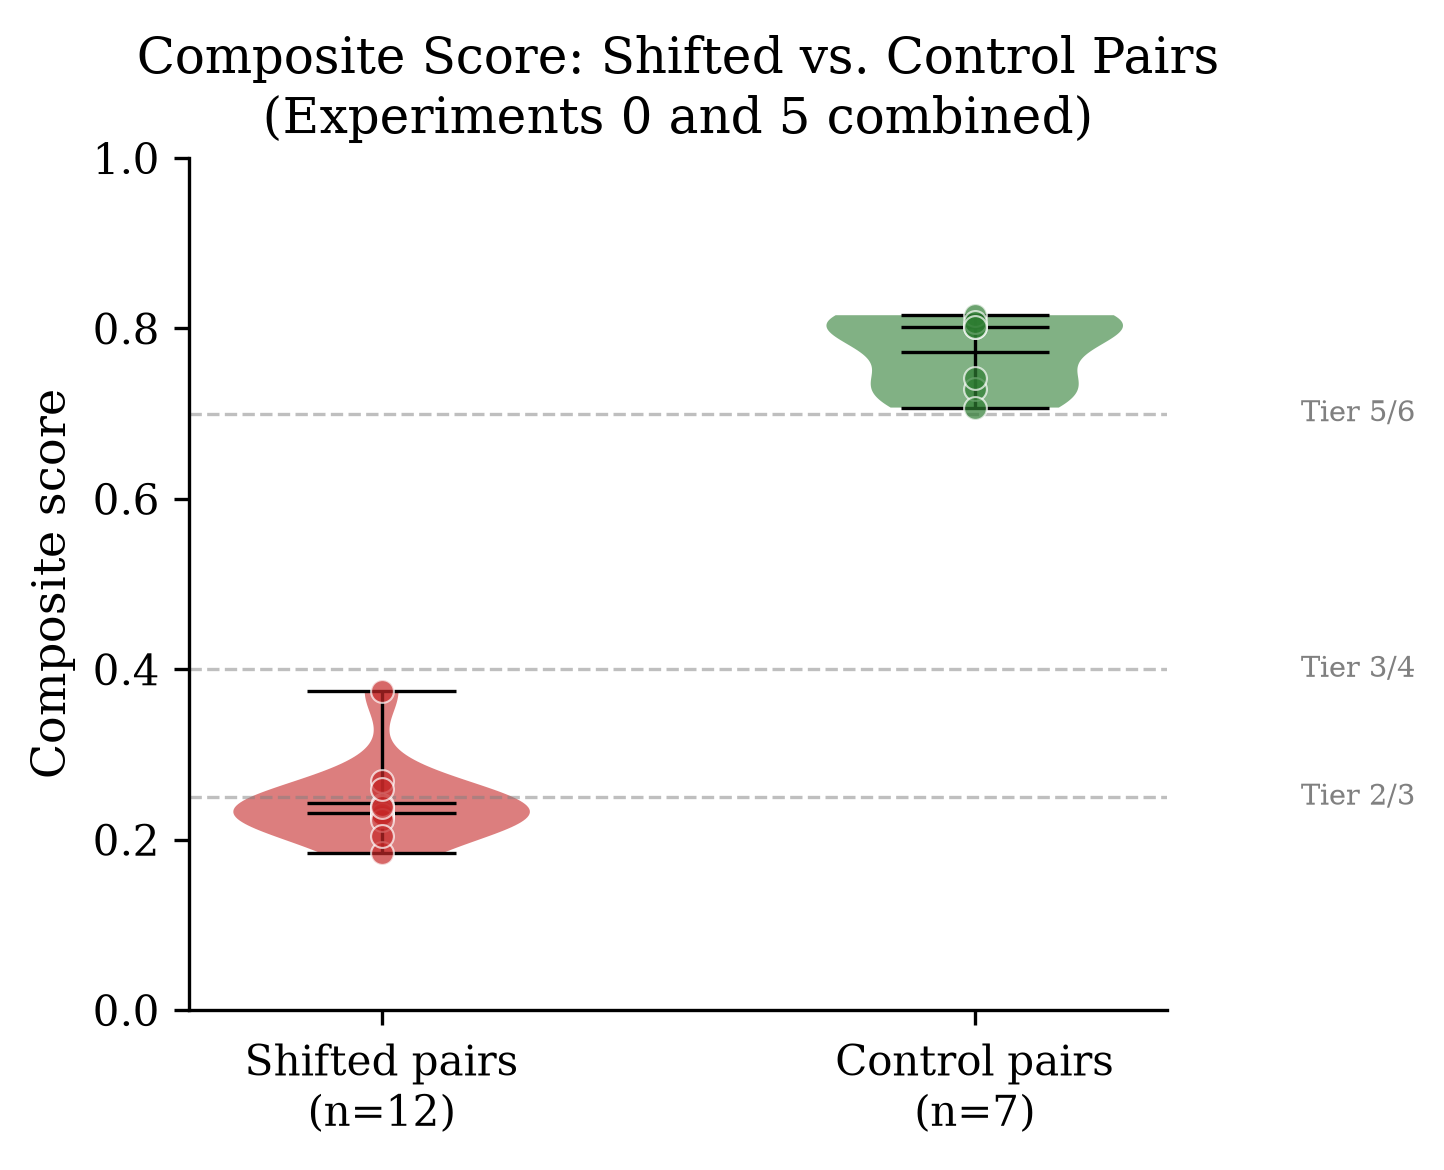
\includegraphics[width=0.48\textwidth]{figures/composite_distributions.pdf}
\caption{Composite score distributions for cross-assay (shifted, $n=12$) and within-assay (control, $n=7$) pairs. The tier gap ($\geq 2$) has zero overlap. Bag-of-genes PCA scores Tier~5--6 on the same shifted conditions (Table~\ref{tab:separation}), indicating that the composite tracks geometric reorganization rather than embedding quality.}
\label{fig:composite}
\end{figure}

This separation is necessary but insufficient: any distributional-shift detector (MMD, C2ST, a two-sample $t$-test) achieves it. The telling observation is in Table~\ref{tab:separation}: bag-of-genes PCA, a no-learned-parameter baseline, scores Tier~5--6 on the same cross-assay conditions where Geneformer scores Tier~2--3. The composite detects that trained models have reorganized their embedding spaces under assay shift. It misses that this reorganization accompanies richer biological encoding---the composite interprets a sign of quality as a deficiency. This is the gap the construct-validity protocol is designed to catch.

\subsection{Check 1: Null-model discrimination}

The first construct-validity check asks whether the metric can distinguish trained embeddings from random projections (Table~\ref{tab:v6b}). At $n = 2{,}000$ cells and $d = 512$, the Johnson--Lindenstrauss regime is approximately satisfied: the standard bound requires $d \geq C \log n / \varepsilon^2$, giving $d \approx 760$ at $\varepsilon = 0.1$ (above $d = 512$) but $d \approx 528$ at $\varepsilon = 0.12$ (below it). Random linear maps at $d = 512$ therefore preserve pairwise distances to $(1 \pm 0.12)$, and with them, any metric that depends on distances, covariance structure, or $k$-nearest-neighbor graphs.

M1 (subspace alignment) and M6 (graph curvature) fail this check. Random projections achieve \emph{higher} M1 scores than trained models ($+1.5$ tier gap, wrong direction) because JL preservation guarantees that covariance eigenspaces are approximately invariant under random linear maps. M6 (Ollivier--Ricci curvature on $k$-NN graphs) similarly cannot distinguish random from trained: JL distance preservation implies neighbor preservation implies curvature preservation. M3 (direction stability) passes: trained models score $+1.5$ tiers above random because random directions are unstable (the Marchenko--Pastur spectrum makes eigenvectors arbitrary). M2 (domain separability) and M4 (participation ratio) pass this check.

Against the structured null (bag-of-genes PCA at matched $d = 512$), the composite fails on both held-out tissues. On liver, the mean composite score of trained 512d models (Geneformer 0.323, scGPT 0.279) exceeds BoG (0.303) by a margin whose bootstrap 95\% CI includes zero ($[-0.024, 0.186]$). On kidney, the point estimate is \emph{negative}: BoG (0.322) exceeds both Geneformer (0.230) and scGPT (0.267). At matched dimensionality, the composite cannot distinguish trained foundation models from $\log(1+x)$ followed by PCA.

\begin{table}[t]
\centering
\caption{Null-model discrimination on held-out tissues. The composite beats random projections (floor: CI excludes zero) but cannot distinguish trained 512d models from bag-of-genes PCA (primary: CI includes zero on liver; point estimate negative on kidney). scVI ($d = 50$) is excluded from the matched-dimensionality comparison.}
\label{tab:v6b}
\small
\begin{tabular}{@{}llccc@{}}
\toprule
Model & Type & $d$ & Liver score & Kidney score \\
\midrule
Random projection & null & 512 & 0.050 & 0.076 \\
Untrained encoder & null & 512 & 0.061 & 0.060 \\
\midrule
Bag-of-genes PCA & structured null & 512 & 0.303 & 0.322 \\
\midrule
Geneformer & trained & 512 & 0.323 & 0.230 \\
scGPT & trained & 512 & 0.279 & 0.267 \\
scVI & trained & 50 & 0.489 & 0.427 \\
\bottomrule
\end{tabular}
\end{table}

scVI ($d = 50$) is the only model that clearly exceeds BoG on both tissues (0.489 vs.\ 0.303 on liver; 0.427 vs.\ 0.322 on kidney). This apparent success cannot be cited as evidence that the composite works, because the same normalization artifacts diagnosed by Check~2 (\S\ref{sec:check2}) create favorable bias at low dimension. Comparing a 50-dimensional embedding against a 512-dimensional baseline reintroduces the dimensionality confound rather than controlling it.

\subsection{Check 2: Cross-dimensionality robustness}
\label{sec:check2}

The second check asks whether the metric ranks embeddings consistently across dimensions. M4 (participation ratio) fails. M4 computes PR $= (\sum \lambda_i)^2 / \sum \lambda_i^2$ on the singular values of the embedding matrix, then normalizes by dividing by $d$. At high embedding dimension, even embeddings with substantial spectral structure produce raw PR values ($\sim 7$--$20$) that, divided by $d = 1280$, land below the 0.01 scoring threshold. UCE ($d = 1280$) floors on three of four tissues: liver (PR$/d = 0.0055$), kidney ($0.0062$), brain ($0.0085$). The same raw spectral structure scores normally at $d = 512$ (all PR$/d > 0.016$) and trivially at $d = 50$ (PR$/d > 0.14$). The module penalizes high-dimensional embeddings regardless of their actual spectral properties---a normalization artifact. The fix (normalizing by effective rank rather than $d$) is straightforward but requires fresh preregistration. The principle generalizes: any metric whose score depends on a hyperparameter of the embedding method (dimension, vocabulary size, number of layers) rather than a property of the embedding itself will produce confounded cross-architecture comparisons.

\subsection{Check 3: Sign-correctness of transfer correlation}

The third check asks whether the metric correlates with downstream performance in the correct direction. M1 and M2 fail (Table~\ref{tab:probes}).

\paragraph{M1 (subspace alignment): anti-predicts transfer.} Within the 512-dimensional panel ($n = 12$ conditions: 3 models $\times$ 4 tissues), M1 anti-predicts transfer: $\rho = -0.76$ (permutation $p = 0.005$) against average probe F1. Models with better-aligned subspaces have \emph{worse} downstream performance at fixed dimension. M1 tracks the wrong thing: alignment is high when both embeddings are dominated by the same low-rank structure (as in BoG-PCA), regardless of whether that structure encodes biology.

\paragraph{M2 (domain separability): anti-predicts transfer.} After fixing a silent-exception bug, the corrected M2 still anti-predicts kNN transfer F1: $\rho = -0.58$ (permutation $p = 0.008$, $n = 20$ conditions). Foundation models that encode rich biology necessarily encode batch effects; richer embeddings are simultaneously more separable and more useful. A metric that penalizes domain separability penalizes representation quality---a structural parallel to the accuracy-fairness tension in fair ML \citep{chouldechova2017impossibility}, where penalizing awareness of a correlated attribute degrades performance on the target task.

\paragraph{M3 (direction stability): passes but power is insufficient.} M3's transfer correlation is $\rho = +0.30$ (95\% CI $[-0.34, +0.80]$, $n = 12$)---the correct sign but statistically indistinguishable from zero. At the same $n$, M1's anti-prediction ($\rho = -0.76$) reaches significance because its effect size is larger; both estimates carry wide confidence intervals. M3 is the sole module that passes all three checks, though it survives by absence of disconfirmation rather than positive confirmation: no identified confound kills it, but its predictive power remains unestablished. M3 has not been tested standalone against BoG; we flag this as a limitation rather than running the test post hoc, because the matched-dimensionality comparison requires fresh preregistration. Standard power analysis indicates that detecting $\rho = 0.30$ as the minimum effect size of scientific interest---a correlation strong enough to provide actionable ranking information---at 80\% power ($\alpha = 0.05$, two-sided) requires $n \approx 85$ conditions, achievable by expanding from 3 to $\sim$7 models at fixed $d$ across 12 tissues.

\subsection{The construct-validity scorecard}

Table~\ref{tab:scorecard} summarizes the protocol's results across all five modules.

\begin{table}[t]
\centering
\caption{Construct-validity scorecard. Each module fails a different check. M3 passes all three but its predictive value is undetermined at current sample size ($n = 12$).}
\label{tab:scorecard}
\small
\begin{tabular}{@{}lcccc@{}}
\toprule
Module & Check 1 (null discrim.) & Check 2 (cross-$d$) & Check 3 (sign) & Status \\
\midrule
M1 (alignment) & \textbf{fail} (JL confound) & pass & \textbf{fail} ($\rho = -0.76$) & Dead \\
M6 (curvature) & \textbf{fail} (JL confound) & pass & -- & Dead \\
M4 (participation ratio) & pass & \textbf{fail} (PR/$d$ artifact) & -- & Dead \\
M2 (domain shift) & pass & pass & \textbf{fail} ($\rho = -0.58$) & Dead \\
M3 (direction stability) & pass & pass & pass (underpowered) & Sole survivor \\
\bottomrule
\end{tabular}
\end{table}

\subsection{The dissociation between transportability and quality}

The sharpest empirical finding is a consistent dissociation between geometric transportability and downstream utility (Table~\ref{tab:dissociation}). Geneformer achieves the highest cell-type probe F1 in 2 of 4 tissues (lung: 0.638, liver: 0.649) and is competitive in the other two (kidney: 0.654 vs.\ scGPT 0.683; brain: 0.633 vs.\ scVI 0.684), yet scores the worst transportability tiers (2--3) in every tissue. Bag-of-genes PCA achieves the best tiers (5--6) but the worst F1 (0.21--0.31). The dissociation holds across all tissues and all embeddings tested---a structural relationship between representation richness and geometric portability.

\begin{table}[t]
\centering
\caption{Transportability and representation quality are inversely related. Geneformer and the other top-F1 models score the worst tiers; BoG has the best tiers and worst F1. Bold: highest F1 per tissue. Transfer F1 is macro-averaged cell-type F1 trained on source, evaluated on target.}
\label{tab:dissociation}
\small
\begin{tabular}{@{}lcccccccc@{}}
\toprule
 & \multicolumn{2}{c}{Geneformer} & \multicolumn{2}{c}{scVI} & \multicolumn{2}{c}{scGPT} & \multicolumn{2}{c}{BoG-512} \\
\cmidrule(lr){2-3}\cmidrule(lr){4-5}\cmidrule(lr){6-7}\cmidrule(lr){8-9}
Tissue & Tier & F1 & Tier & F1 & Tier & F1 & Tier & F1 \\
\midrule
Lung   & 3 & \textbf{0.638} & 4 & 0.550 & 3 & 0.300 & 5 & 0.304 \\
Liver  & 2 & \textbf{0.649} & 3 & 0.398 & 2 & 0.368 & 5 & 0.228 \\
Kidney & 2 & 0.654 & 3 & 0.454 & 3 & \textbf{0.683} & 5 & 0.306 \\
Brain  & 2 & 0.633 & 3 & \textbf{0.684} & 3 & 0.447 & 6 & 0.208 \\
\bottomrule
\end{tabular}
\end{table}

This dissociation illustrates why the protocol matters. The composite measures geometric reorganization of the embedding space under assay shift---something real. Models that encode more biology also encode more assay-specific variance, producing larger subspace rotations, higher domain separability, and lower composite scores. This geometric signal has a dual interpretation: from a validity standpoint, the composite anti-predicts transfer quality; from a diagnostic standpoint, it correctly identifies that Geneformer's embedding space encodes assay-specific variance that a practitioner might want to address through domain adaptation or fine-tuning. The protocol does not dismiss this diagnostic value---it flags that the composite cannot serve double duty as both a diagnostic tool and a quality ranking. Without the sign-correctness check, this dual role is invisible: the metric appears to rank embedding quality while actually tracking a property (geometric reorganization) that correlates negatively with the outcome practitioners optimize. The protocol catches this because Check~3 directly tests whether the metric rewards what users want to optimize.

\subsection{Existing scalar metrics also lack predictive validity}

Existing shift-detection metrics face the same gap (Table~\ref{tab:scalar}). C2ST achieves near-perfect separation between shifted and control pairs (shifted AUC $> 0.97$; control $\approx 0.50$) but provides no gradient among shifted conditions: all five Geneformer shifted pairs score within a 2.6 percentage-point range. RankMe effective rank difference varies 12-fold across shifted pairs ($3.4$--$42.6$) without monotonic correspondence to downstream degradation---brain cross-assay (RankMe~$= 36.2$) has the smallest degradation (0.164), while lung (RankMe~$= 3.4$) has comparable degradation (0.171). These metrics detect distributional difference---the easy test---without predicting downstream impact. The protocol's Check~3 would flag all of them.

\begin{table}[t]
\centering
\caption{Scalar shift metrics on 9 Geneformer embedding pairs (5 shifted, 4 control). All detect shift but none monotonically tracks degradation. Check~3 (sign-correctness) would flag all of them.}
\label{tab:scalar}
\small
\begin{tabular}{@{}llccccc@{}}
\toprule
Pair & Type & Degrad. & Tier & RankMe $\Delta$ & MMD & C2ST \\
\midrule
Lung (assay)  & shifted & 0.171 & 3 & 3.4  & 0.175 & 0.979 \\
Liver (assay) & shifted & 0.321 & 2 & 3.7  & 0.334 & 0.999 \\
Brain (assay) & shifted & 0.164 & 2 & 36.2 & 0.526 & 0.982 \\
Brain$\to$Lung  & shifted & 0.175 & 2 & 24.9 & 0.285 & 0.985 \\
Liver$\to$Lung  & shifted & 0.196 & 2 & 42.6 & 0.277 & 0.973 \\
\midrule
Lung (ctrl)   & control & -- & 6 & 0.8 & 0.018 & 0.491 \\
Liver (ctrl)  & control & -- & 6 & 1.5 & 0.026 & 0.497 \\
Kidney (ctrl) & control & -- & 6 & 1.0 & 0.012 & 0.493 \\
Brain (ctrl)  & control & -- & 6 & 0.3 & 0.019 & 0.502 \\
\bottomrule
\end{tabular}
\end{table}

\subsection{The field-standard scIB suite passes the easy test and fails the hard one}
\label{sec:scib}

We applied the construct-validity protocol to the full scIB metric suite \citep{luecken2022scib} under a separate preregistration (SHA-256--frozen scorer and hypothesis routing before data access). Ten metrics were testable: five bio-conservation (NMI, ARI, silhouette-label, cLISI, isolated-label ASW) and five batch-correction (silhouette-batch, iLISI, kBET, graph connectivity, PCR comparison). Six embeddings (Geneformer, scVI, scGPT, bag-of-genes PCA-512, random projection, untrained encoder) were evaluated across four tissues ($n = 2{,}000$ per side, seed distinct from the main study). Ground-truth transfer performance is macro-averaged cell-type kNN F1 from source to target.

\paragraph{Choice of ground truth.} We use cross-assay cell-type classification F1 as the validity anchor because it captures the practitioner's deployment question: ``which embedding will generalize to new assay conditions?'' scIB was designed for a different question---``did batch integration work?''---and may be appropriate for that use case. Our claim is narrower than ``scIB is broken'': scIB metrics lack predictive validity for cross-assay transferability, the question that current foundation model benchmarks use them to answer. A metric that is valid for integration evaluation may still be invalid when repurposed for model ranking.

\paragraph{Check 1 (null-model discrimination).} Eight of nine testable metrics pass: trained embeddings score significantly higher than null models, with bootstrap 95\% CIs excluding zero. The largest effects are graph connectivity ($\Delta = 0.49$, CI $[0.45, 0.54]$) and NMI ($\Delta = 0.23$, CI $[0.14, 0.31]$). PCR comparison fails (CI $[-0.03, 0.46]$ includes zero; 16 of 24 conditions returned exactly 0.0). kBET returned null for all 24 conditions and was scored N/A---an applicability limit under cross-assay batch structure, not a metric flaw. This confirms that scIB metrics reliably distinguish trained from random. The question is whether that capability extends to ranking the trained models a practitioner chooses among.

\paragraph{Pairwise ranking accuracy on contenders.} To test the harder question---\emph{which} trained model to deploy---we defined a ``contenders'' set: Geneformer, scVI, scGPT, and bag-of-genes PCA-512, the models a practitioner would compare (nulls excluded because ``is it trained?'' is not the deployment question). Within each tissue, we counted pairwise rank inversions against ground-truth F1 (6 pairs per tissue, 24 total). An inversion occurs when the metric ranks embedding A above B but F1 ranks B above A.

Every bio metric inverts 46--58\% of contender comparisons, with tissue-clustered bootstrap 95\% CIs whose lower bounds reach or exceed 50\% (Table~\ref{tab:scib_inversions}, Figure~\ref{fig:inversions}). Cross-tissue stability is simultaneously high: Kendall's $W > 0.80$ for all bio metrics, meaning the inversions are consistent across tissues. The metrics produce a confident, reproducible ordering that does not track downstream performance.

\begin{table}[t]
\centering
\caption{Pairwise inversion rate against ground-truth F1 on the contenders-4 condition set (6 pairs $\times$ 4 tissues $= 24$ comparisons), split by F1 gap. Clear winners ($|\Delta\text{F1}| > 0.10$): the metric's ranking call matters. Near-ties ($|\Delta\text{F1}| \leq 0.10$): the correct ranking is ambiguous. Tissue-clustered bootstrap 95\% CI on the overall rate. All results are exploratory.}
\label{tab:scib_inversions}
\small
\begin{tabular}{@{}lccccc@{}}
\toprule
 & \multicolumn{2}{c}{Clear winners} & \multicolumn{2}{c}{Near-ties} & Overall \\
\cmidrule(lr){2-3}\cmidrule(lr){4-5}
Metric & inv / $n$ & rate & inv / $n$ & rate & rate [95\% CI] \\
\midrule
NMI       & 2/10 & 0.20 & 9/14  & 0.64 & 0.46 [0.33, 0.58] \\
ARI       & 0/10 & 0.00 & 11/14 & 0.79 & 0.46 [0.33, 0.58] \\
Sil-label & 2/10 & 0.20 & 11/14 & 0.79 & 0.54 [0.50, 0.63] \\
cLISI     & 2/10 & 0.20 & 12/14 & 0.86 & 0.58 [0.42, 0.75] \\
Iso-label & 2/10 & 0.20 & 12/14 & 0.86 & 0.58 [0.50, 0.67] \\
\bottomrule
\end{tabular}
\end{table}

\begin{figure}[tb]
\centering
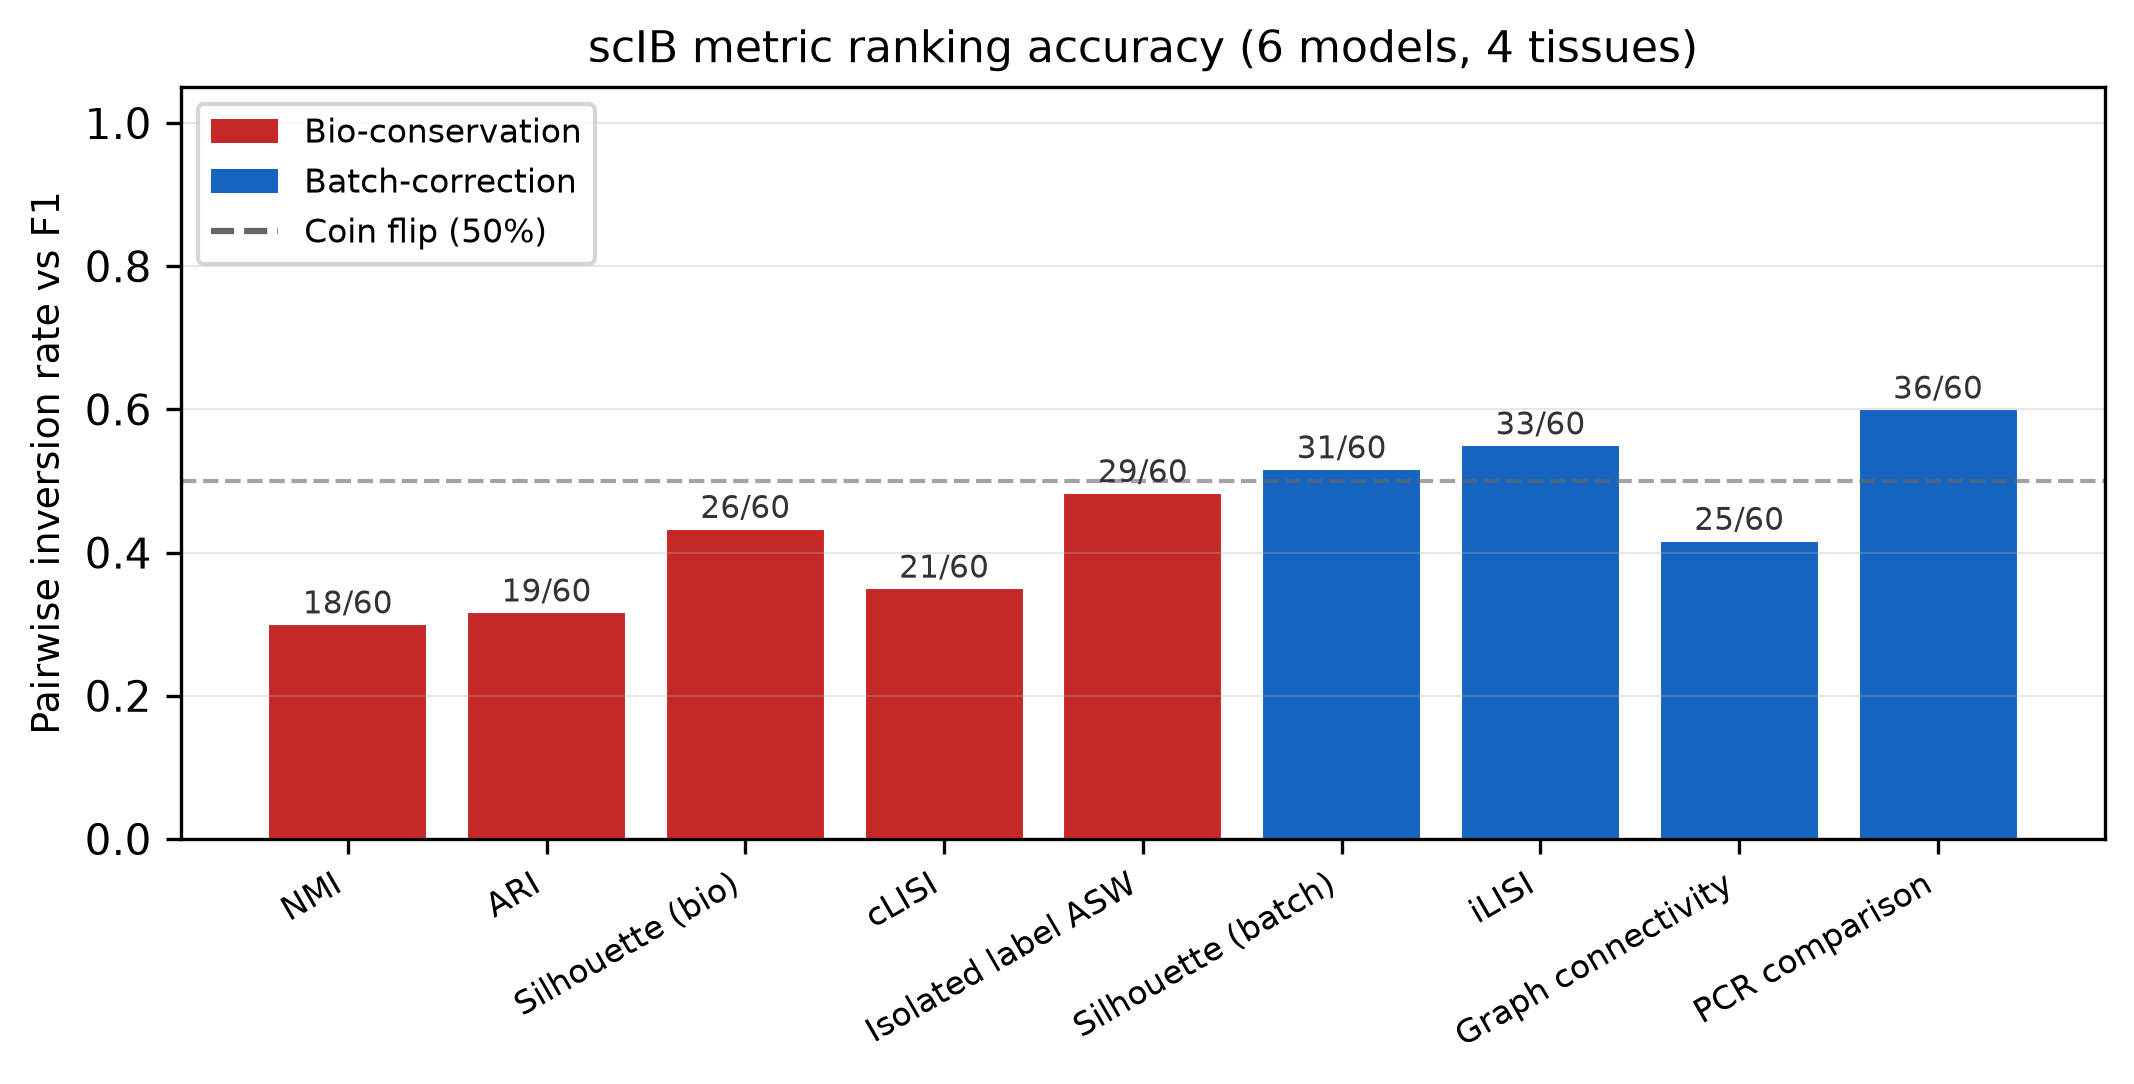
\includegraphics[width=0.7\textwidth]{figures/inversion_rates.pdf}
\caption{Pairwise inversion rates against ground-truth transfer F1 on the contenders set (4 embeddings, 6 pairs $\times$ 4 tissues $= 24$ comparisons). Bio-conservation metrics (red) invert 46--58\% of comparisons; batch-correction metrics (blue) range from 46\% to 67\%. Dashed line: coin flip. kBET excluded (all null).}
\label{fig:inversions}
\end{figure}

\paragraph{Three tiers of predictive accuracy.} The F1-gap split reveals a graded pattern (Table~\ref{tab:scib_inversions}). \emph{Pick-the-winner}: scIB metrics correctly identify the best-performing model (Geneformer) at 80--100\% accuracy on clear-gap comparisons ($|\Delta\text{F1}| > 0.10$); Clopper--Pearson 95\% CIs for the clear-winner accuracy range from $[0.44, 0.97]$ (8/10) to $[0.69, 1.00]$ (10/10), so even the best-case metric cannot rule out near-chance accuracy with $n = 10$ clear-gap pairs. \emph{Rank-the-field}: among the remaining models (scVI, scGPT, BoG-PCA), all 14 near-tie comparisons hit 64--86\% inversion rates---worse than chance. \emph{Beat-the-baseline}: the two clear-gap inversions that exist are both kidney, where scVI and scGPT score higher than BoG-PCA on every bio metric while BoG-PCA achieves 0.15--0.20 higher transfer F1. The metrics confidently prefer trained models over a no-learned-parameter baseline that actually transfers better---an existence proof that the suite can be wrong on a clear gap, not merely unable to resolve ties.

The mechanism is the same one identified for our own modules (\S\ref{sec:check2}): scIB bio metrics reward cluster compactness of known cell types, a property that trained-versus-random separates easily. Ranking two competent embeddings by transfer quality requires sensitivity to cross-assay alignment---a property the suite's integration-oriented design never optimized for. The suite was designed to evaluate batch correction (``did integration work?'') and succeeds at that task; it was not designed to rank embeddings by cross-assay transferability, and fails when repurposed for that question.

\paragraph{Implications for published benchmark conclusions.} These inversion rates have concrete consequences for published results. \citet{wu2025scfm} concluded that Geneformer ``excels at transfer learning tasks'' based partly on scIB bio-conservation scores; our analysis confirms that Geneformer does achieve the best transfer F1 on clear-gap comparisons, but scIB metrics reach this conclusion for the wrong reason (cluster compactness, not transfer quality) and would give the same ranking to any model that happens to produce compact clusters. VCBench \citep{vcbench2026} reports a single scIB overall score averaging bio and batch axes; our redundancy analysis (below) shows that this average double-counts the NMI--ARI signal and dilutes it with inoperative batch metrics, potentially masking tissue-specific ranking failures like the kidney inversion documented above. These are not hypothetical concerns: the kidney inversion (Table~\ref{tab:dissociation}) would direct a practitioner to deploy a model with 0.15--0.20 lower transfer F1 than the baseline.

\paragraph{Suite redundancy.} Pairwise Spearman correlation across 24 conditions reveals that the 10-metric suite has approximately 3--4 independent signals. NMI and ARI are near-identical ($\rho = 0.91$); cLISI is rank-redundant with NMI ($\rho = 0.86$) despite having almost no dynamic range (all scores $> 0.90$, wrong-sign Check~3 correlation). The effective bio-conservation signal is carried by NMI-or-ARI plus silhouette-label; the effective batch signal is graph connectivity alone (iLISI near-zero everywhere, PCR comparison undefined on most conditions). Reporting a single ``scIB overall score'' as a weighted average of 10 metrics double-counts the NMI--ARI axis, dilutes signal with inoperative batch metrics, and collapses a genuine bio--batch tradeoff into a single scalar.

\paragraph{Epistemic status.} Check~1 and the per-metric routing were preregistered. The inversion analysis, F1-gap split, redundancy analysis, and three-tier characterization are exploratory---computed after viewing Check~1 results. We tested a summary-statistic version of the dissociation hypothesis (Spearman correlation between Check~1 $\Delta$ and Check~3 $\rho$ across 5 bio metrics) and it did not hold ($\rho = +0.70$, $p = 0.19$, $n = 5$); the direct pairwise-inversion measurement reported above replaced it. Both confirmatory tests---hyperparameter sensitivity and noise dose-response---have been executed (below).

\paragraph{Hyperparameter sensitivity (confirmatory).} We preregistered predictions for how Leiden resolution ($r \in \{0.5, 1.0, 2.0\}$) and kNN neighborhood size ($k \in \{15, 30, 90\}$) would affect metric rankings, then executed the test on SHA-256--frozen scorer code (Table~\ref{tab:hyperparam}). For each metric, we computed Kendall's $\tau$ between the embedding ranking at the most extreme hyperparameter pair across four tissues. The preregistration predicted substantial instability: NMI $\tau \in [0.5, 0.7]$, ARI $\tau \in [0.4, 0.6]$, cLISI $\tau \in [0.3, 0.6]$, graph connectivity $\tau \in [0.3, 0.6]$, kBET $\tau \in [0.1, 0.4]$, iLISI $\tau \in [0.2, 0.5]$. All six predictions were wrong in the same direction: every computable metric is far more stable than predicted. NMI rankings are perfectly preserved in three of four tissues ($\tau = 1.0$; mean extreme $\tau = 0.93$). ARI shows the largest variation ($\tau = 0.47$ in brain, one winner change across four tissues) but still exceeds its predicted ceiling. Ranking divergence accumulates gradually: adjacent-pair $\tau$ values (e.g., $r = 0.5$ vs.\ $1.0$, or $r = 1.0$ vs.\ $2.0$) are uniformly $\geq 0.73$ for NMI and $\geq 0.47$ for ARI (Appendix~\ref{app:hyperparam}, Table~\ref{tab:app_tau}), confirming that the extreme-pair comparison is not cherry-picked. cLISI and graph connectivity are near-perfectly stable (mean extreme $\tau \geq 0.93$). kBET returned null for all conditions (consistent with the exploratory audit), and iLISI was near-zero for most conditions, making $\tau$ undefined. Only 1 of 16 metric $\times$ tissue combinations produced a winner change (ARI in brain, where scVI and Geneformer swap at resolution 2.0).

\begin{table}[t]
\centering
\caption{Hyperparameter sensitivity (confirmatory). Kendall's $\tau$ between embedding rankings at extreme hyperparameter settings (Leiden $r = 0.5$ vs $2.0$; kNN $k = 15$ vs $90$), across four tissues. All predictions underestimated stability. kBET returned null for all conditions; iLISI near-zero for most, making $\tau$ undefined. 0/6 predictions in range.}
\label{tab:hyperparam}
\small
\begin{tabular}{@{}lcccccc@{}}
\toprule
 & \multicolumn{4}{c}{Extreme-pair $\tau$} & Mean & Predicted \\
\cmidrule(lr){2-5}
Metric & Lung & Liver & Kidney & Brain & $\bar{\tau}$ & range \\
\midrule
NMI & 1.00 & 1.00 & 1.00 & 0.73 & 0.93 & 0.5--0.7 \\
ARI & 0.87 & 0.87 & 1.00 & 0.47 & 0.80 & 0.4--0.6 \\
cLISI & 1.00 & 0.97 & 0.87 & 1.00 & 0.96 & 0.3--0.6 \\
Graph conn. & 0.87 & 1.00 & 0.87 & 1.00 & 0.93 & 0.3--0.6 \\
iLISI & 0.58 & 0.67 & NaN & NaN & NaN & 0.2--0.5 \\
kBET & \multicolumn{4}{c}{all null} & N/A & 0.1--0.4 \\
\bottomrule
\end{tabular}
\end{table}

This result strengthens the paper's central finding. The 46--58\% pairwise inversion rates against F1 (Table~\ref{tab:scib_inversions}) are not artifacts of hyperparameter choice---the metrics produce the same rankings regardless of whether Leiden resolution is 0.5 or 2.0, or whether kNN uses $k = 15$ or $k = 90$. The inversions documented in the exploratory analysis are genuine properties of the metrics, reproducible across hyperparameter settings, not sensitivity to implementation details.

\paragraph{Noise dose-response (confirmatory).} We preregistered predictions for how additive Gaussian noise at $\sigma \in \{0.01, 0.05, 0.1, 0.25, 0.5, 1.0, 2.0\} \times \text{embedding\_std}$ would affect each metric's monotonicity across 24 conditions (4 tissues $\times$ 6 embeddings). A metric FAILS if non-monotonic in more than 1 of 24 conditions (Table~\ref{tab:noise}). The threshold of $>1$ (rather than $>0$) was preregistered to allow for numerical noise: a single reversal smaller than $10^{-3}$ could reflect floating-point artifacts rather than genuine non-monotonicity. Under a binomial null where reversals occur by chance at rate $p = 0.05$ (one-in-twenty conditions), observing $>1$ of 24 has probability $< 0.01$, so the threshold is conservative against false positives.

The results split cleanly along the bio/batch axis (Table~\ref{tab:noise}, Figure~\ref{fig:noise}). Every bio-conservation metric fails: NMI (17/24 non-monotonic), ARI (22/24), cLISI (11/24), isolated-label ASW (9/24), and silhouette-label (3/24). Both batch-correction metrics with computable values pass: silhouette-batch and pcr-comparison increase monotonically in 23/24 conditions. iLISI (2/24 non-monotonic) and graph connectivity (22/24) also fail. kBET returned null for all 168 evaluations. This reflects an applicability limit specific to kBET: its permutation test requires sufficient within-label batch heterogeneity, which the two-label cross-assay design does not provide. Other batch metrics (silhouette-batch, iLISI) compute under the same design without difficulty. Preregistered predictions matched 4 of 10 outcomes; the six misses all erred in the same direction (predicting stability where metrics were fragile), indicating that our priors systematically underestimated how sensitive bio-conservation metrics are to embedding perturbation. The consistent direction of miscalibration is itself informative: it suggests that the field's intuition about metric robustness---which shaped our priors---overestimates the stability of bio-conservation scores under perturbation. This miscalibration does not affect the confirmatory status of the test, because the pass/fail criterion was preregistered and the predictions were wrong in the conservative direction (predicting PASS where the outcome was FAIL). Graph connectivity is the sharpest surprise: 22/24 conditions are non-monotonic despite near-perfect ranking stability under hyperparameter variation ($\bar{\tau} = 0.93$ in the preceding test).

\begin{table}[t]
\centering
\caption{Noise dose-response (confirmatory). Non-monotonicity count across 24 conditions (4 tissues $\times$ 6 embeddings) at 7 noise levels ($\sigma \in \{0.01, \ldots, 2.0\} \times \text{embedding\_std}$). A metric FAILS if non-monotonic in $>1$ condition. All bio-conservation metrics fail; both computable batch metrics pass. kBET returned null for all 168 evaluations.}
\label{tab:noise}
\small
\begin{tabular}{@{}lcccl@{}}
\toprule
Metric & Non-mono & Predicted & Actual & Direction \\
\midrule
NMI & 17/24 & FAIL & FAIL & --- \\
ARI & 22/24 & FAIL & FAIL & --- \\
Silhouette label & 3/24 & PASS & FAIL & --- \\
cLISI & 11/24 & PASS & FAIL & --- \\
Isolated label ASW & 9/24 & PASS & FAIL & --- \\
\midrule
Silhouette batch & 1/24 & PASS & PASS & $\uparrow$ (23/23 non-decreasing) \\
iLISI & 2/24 & PASS & FAIL & --- \\
kBET & 0/0 & FAIL & PASS$^*$ & all null \\
Graph connectivity & 22/24 & PASS & FAIL & --- \\
PCR comparison & 1/24 & PASS & PASS & $\uparrow$ (23/23 non-decreasing) \\
\bottomrule
\multicolumn{5}{@{}l@{}}{\footnotesize $^*$kBET returned null for all 168 evaluations; PASS is vacuous.}
\end{tabular}
\end{table}

\begin{figure}[tb]
\centering
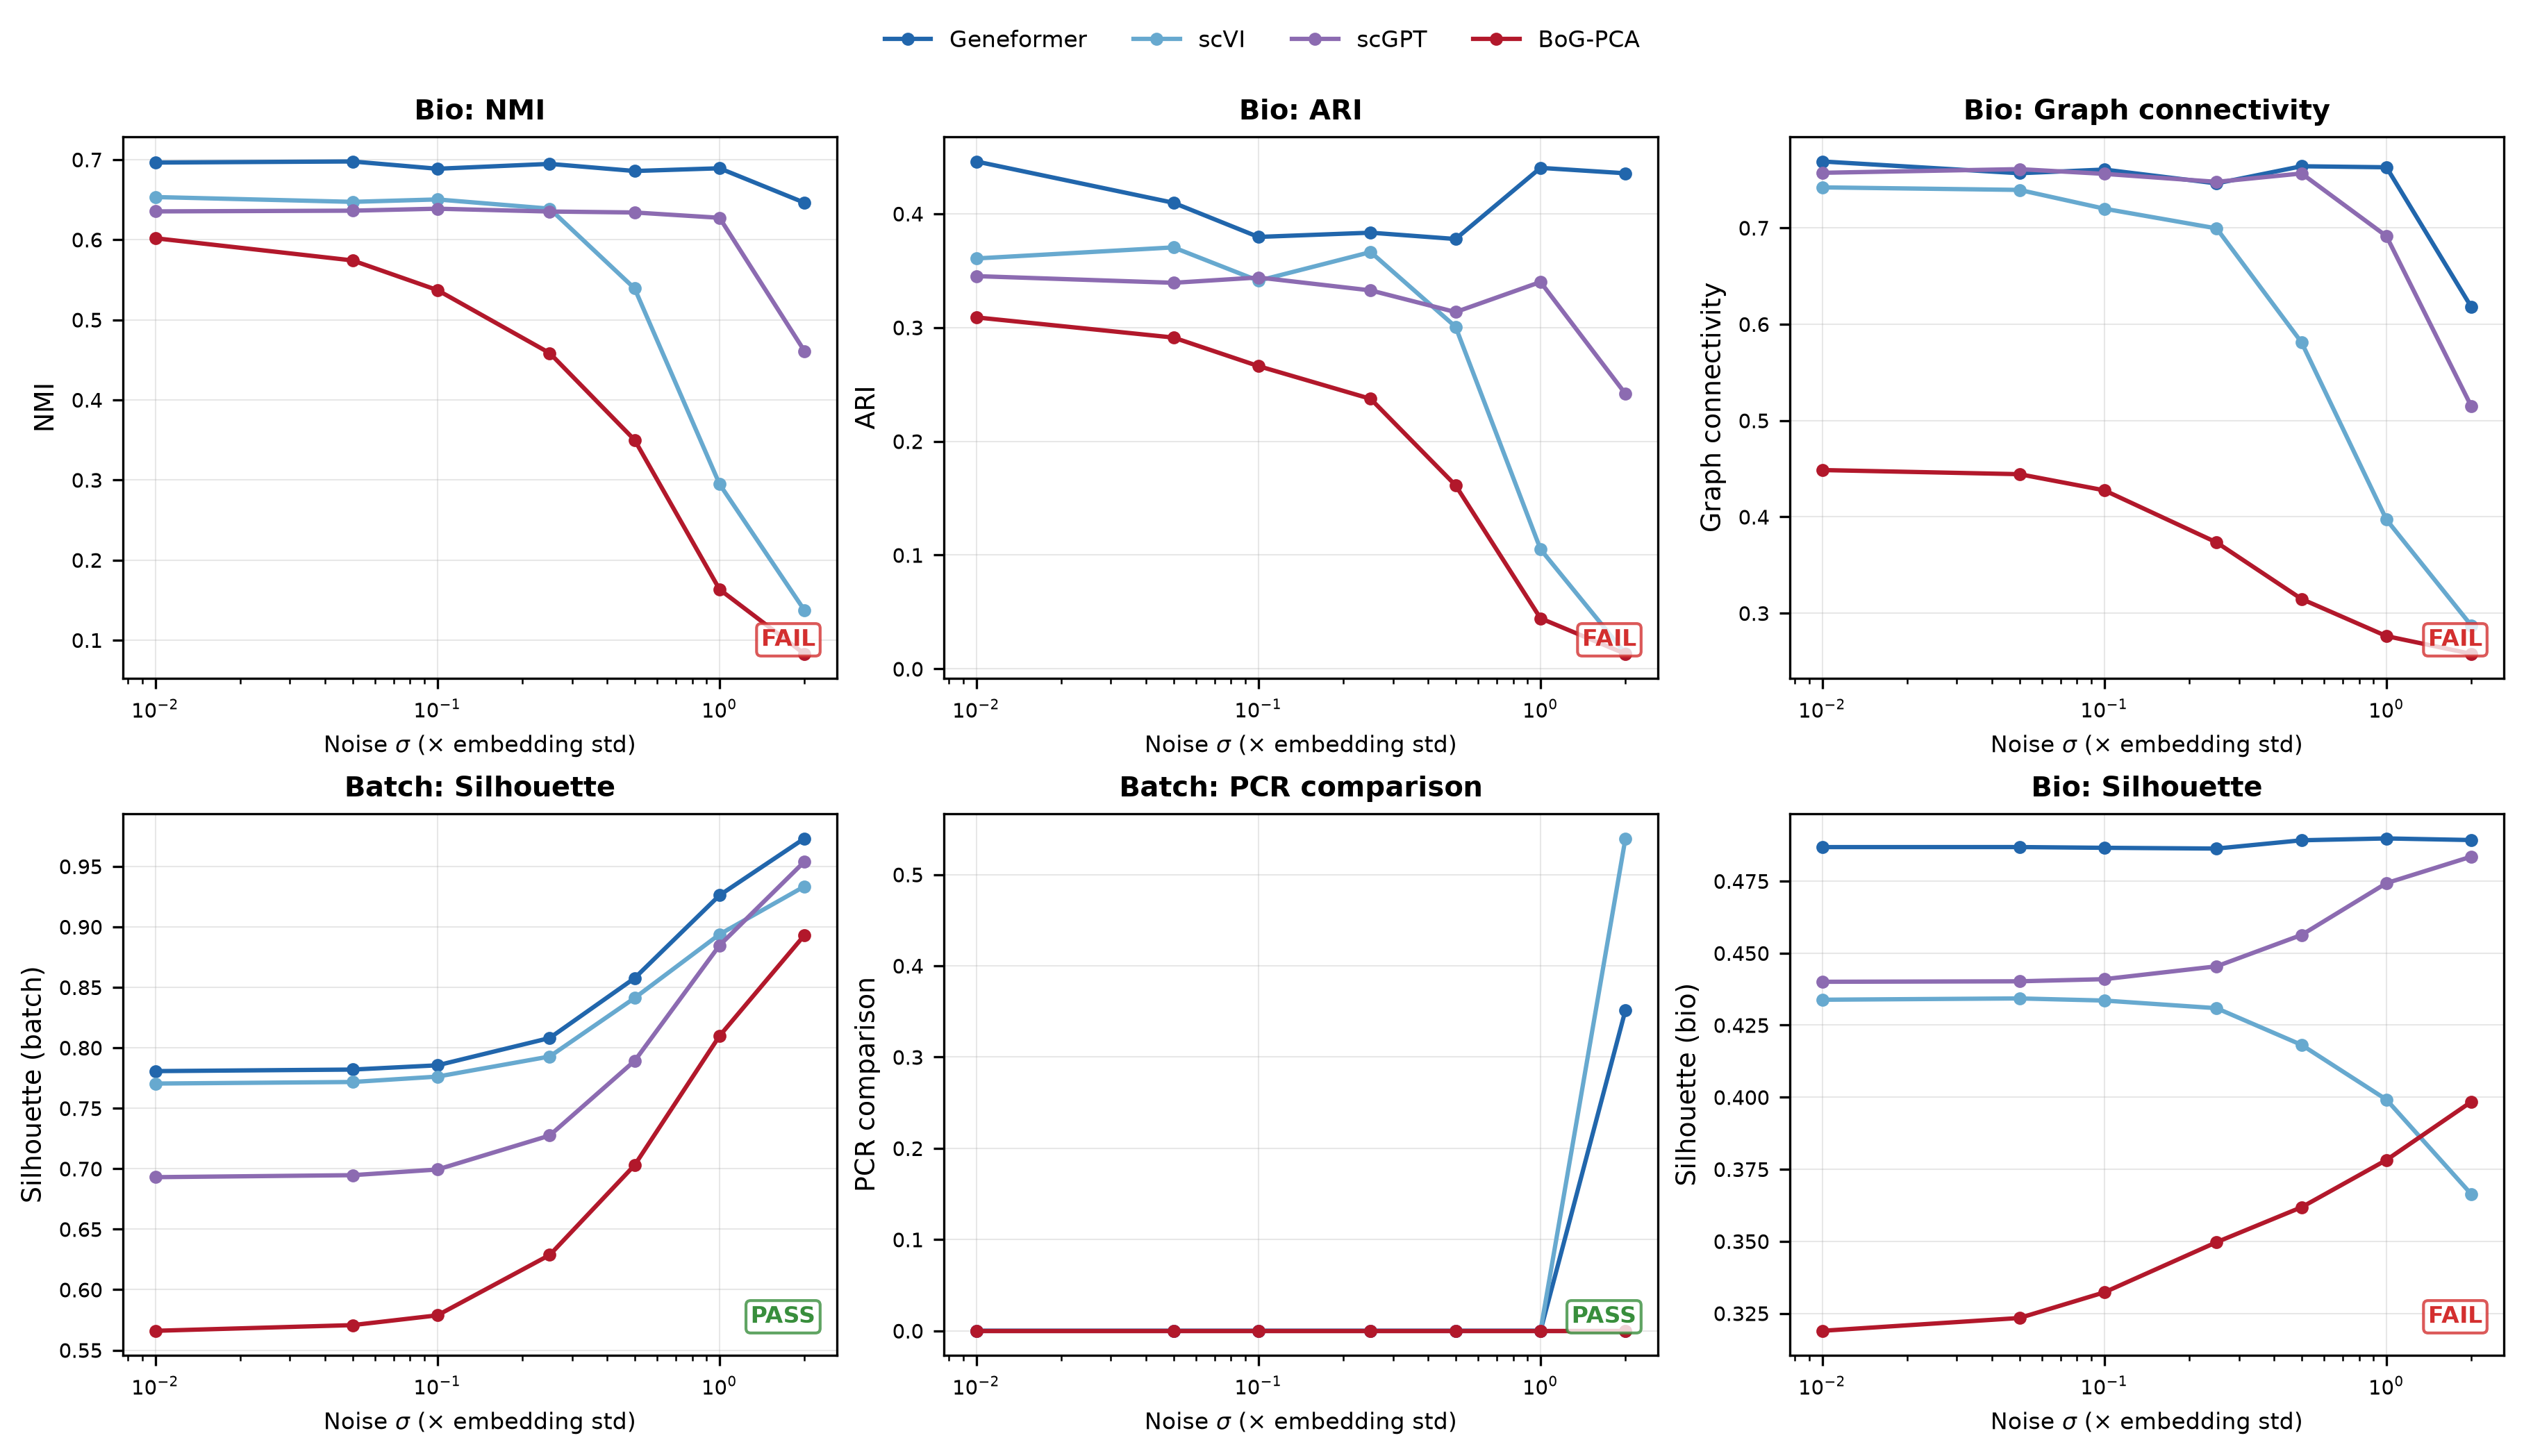
\includegraphics[width=\textwidth]{figures/noise_dose_response.pdf}
\caption{Noise dose-response for six scIB metrics on lung tissue (4 trained embeddings). \textbf{Top}: bio-conservation metrics respond non-monotonically---values increase at intermediate $\sigma$ before collapsing. \textbf{Bottom left}: silhouette-batch increases monotonically (noise destroys batch structure; mechanical PASS). \textbf{Bottom center}: PCR comparison is zero except at $\sigma = 2.0$ (mechanical PASS). $\sigma$ scaled by embedding standard deviation. Full data: Appendix~\ref{app:noise}.}
\label{fig:noise}
\end{figure}

The two confirmatory tests together reveal complementary failure modes. Hyperparameter sensitivity shows that metric \emph{rankings} are stable (inversions are intrinsic, not artifacts); noise dose-response shows that metric \emph{values} are often non-monotonic under controlled degradation. These are independent properties: graph connectivity exhibits the dissociation most sharply, with near-perfect ranking stability ($\bar{\tau} = 0.93$) coexisting with pervasive non-monotonicity (22/24 conditions). Of the original 10 scIB metrics, only silhouette-batch and pcr-comparison survive both tests---and they survive for a mechanical reason. Noise destroys batch-specific structure, so batch-mixing scores improve monotonically as noise increases; the metric moves in the expected direction because the degradation aligns with what the metric rewards, independent of embedding quality. Passing the noise test is necessary but not sufficient for a useful metric: it establishes that the metric responds coherently to quality degradation, without guaranteeing that the metric tracks the right axis of quality. Silhouette-batch and PCR comparison pass because noise mechanically improves what they measure (batch mixing), an alignment that would hold for any perturbation that destroys batch structure, whether or not that perturbation corresponds to meaningful quality change. A fourth check---whether monotonic response corresponds to meaningful quality change---could strengthen the protocol; we leave this for future work. The immediate conclusion is that no scIB metric survives both confirmatory tests as a reliable indicator of \emph{bio-conservation} quality---the axis on which current benchmarks compare models.


\subsection{What the protocol catches and what it misses}

The preceding analyses document which checks each metric fails. Three concrete cases illustrate how these failures would affect a practitioner's decision. All three use criteria defined before the data were examined: the composite tier thresholds (preregistered), Check~3 sign-correctness (preregistered), and the scIB inversion analysis (exploratory, but computed using the preregistered Check~3 criterion). No threshold or gate was adjusted to make any vignette land.

\paragraph{Catch 1: scIB nominates the wrong embedding in kidney.} In kidney, every scIB bio metric (NMI, ARI, silhouette-label, cLISI, isolated-label ASW) ranks scVI and scGPT above bag-of-genes PCA-512. A practitioner consulting the scIB scorecard would select a trained model over the baseline. Ground-truth transfer F1 reverses this ranking: BoG-PCA achieves 0.15--0.20 higher cross-assay F1 than scVI or scGPT in kidney (Table~\ref{tab:dissociation}). These are clear-gap inversions ($|\Delta\text{F1}| > 0.10$), not near-ties. Check~3 catches this directly: a metric whose ranking contradicts transfer performance on a clear gap fails sign-correctness. The practitioner would have deployed the worse embedding.

\paragraph{Catch 2: the composite flags Geneformer for cross-assay deployment.} Standard benchmarks nominate Geneformer: it achieves the highest or near-highest cell-type probe F1 across tissues (0.63--0.65) and the best scIB bio scores. A practitioner choosing an embedding for cross-assay transfer would select it. The composite assigns Tier~2--3 across all four tissues (Table~\ref{tab:dissociation}), flagging Geneformer's embedding space as geometrically reorganized under assay shift. The tier cutoff (Tier~$\leq 3$ = unacceptable for direct transfer) was defined before data access. The composite catches something the benchmarks miss: Geneformer encodes assay-specific variance alongside biology, producing subspace rotations and domain separability that degrade transfer despite strong within-distribution performance. Without the protocol, the deployment risk is invisible.

\paragraph{Miss: the protocol does not catch the BoG-PCA degeneracy.} Bag-of-genes PCA-512 achieves Tier~5--6 on all four cross-assay conditions (Table~\ref{tab:separation}) despite the worst transfer F1 of any embedding tested (0.21--0.31; Table~\ref{tab:dissociation}). The composite scores it as safe because PCA distributes variance across components by construction: M4 reports healthy spectral spread, M1 reports high eigenspace similarity, and M2 is low because PCA does not encode assay identity. The degeneracy is structural---the directions that carry variance do not encode biologically meaningful distinctions---and no geometric module detects this. A practitioner trusting the tier alone would deploy the worst-transferring embedding in the panel. Detecting structural degeneracy requires probing whether geometric properties correspond to biological categories, a role that falls to downstream evaluation rather than geometric diagnostics.

\subsection{Downstream probes are the only reliable predictor}

Across all 20 model $\times$ tissue conditions (5 models $\times$ 4 tissues, including UCE at $d = 1280$), the only quantity that reliably predicts transfer performance is the downstream probe itself (Table~\ref{tab:probes}). No geometric composite---including variants with M4 removed, M6 removed, or different weight schemes---achieves a significant positive correlation with either probe metric.

\begin{table}[t]
\centering
\caption{No geometric metric positively predicts transfer. Spearman correlations with $10{,}000$-resample bootstrap 95\% CIs ($n = 20$: 5 models $\times$ 4 tissues). The only significant correlations are \emph{anti}-predictive (M1, M2). ``ns'' = CI includes zero; ``sig'' = CI excludes zero, confirmed by permutation test.}
\label{tab:probes}
\small
\begin{tabular}{@{}lccc@{}}
\toprule
Metric & vs logreg F1 & vs kNN F1 & vs avg F1 \\
\midrule
Composite (v6) & $-0.01$ ns & $-0.28$ ns & $-0.07$ ns \\
M2+M3 (v6b) & $+0.12$ ns & $-0.15$ ns & $+0.08$ ns \\
M3 alone & $+0.09$ ns & $-0.05$ ns & $+0.09$ ns \\
M2 alone & $-0.24$ ns & $\mathbf{-0.58}$ sig & $-0.36$ ns \\
M1 alone & $-0.45$ ns & $\mathbf{-0.48}$ sig & $\mathbf{-0.54}$ sig \\
\bottomrule
\end{tabular}
\end{table}

The result is robust to dimension control. Within the 512-dimensional panel ($n = 12$: 3 models $\times$ 4 tissues), M1 remains anti-predictive ($\rho = -0.76$, permutation $p = 0.005$). No module achieves a positive significant correlation at any dimensionality. All transfer correlations rest on $n = 12$--$20$ conditions; we state confidence intervals throughout and apply the power caveat symmetrically to both anti-predictive results (M1, M2) and the positive-but-non-significant result (M3).


\section{Methods}

\subsection{Data}

All embeddings are accessed via the CellxGene Census API (v2023-12-15) \citep{abdulla2025cellxgene}. Cross-assay pairs compare 10x Chromium 3' v3 (source) against Smart-seq2 (target) within the same tissue, with zero donor overlap enforced by metadata filtering. Five tissues were initially planned; heart was excluded because Census returned zero Smart-seq2 target cells after metadata filtering, leaving four: lung (191K source, 42K target available), liver (191K source, 42K target), kidney (121K source, 4.3K target), and brain (available counts vary by model). All evaluations subsample $n = 2{,}000$ cells per side. Five embedding methods: Geneformer ($d = 512$) \citep{theodoris2023geneformer}, scGPT ($d = 512$) \citep{cui2024scgpt}, scVI ($d = 50$) \citep{lopez2018scvi}, UCE ($d = 1280$) \citep{rosen2026uce}, and bag-of-genes PCA-512 ($d = 512$; $\log(1 + x)$ without total-count normalization, PCA with fixed seed). Two null baselines: random Gaussian projection ($R \in \mathbb{R}^{512 \times G}$, $R_{ij} \sim \mathcal{N}(0, 1/\sqrt{512})$) and an untrained two-layer MLP encoder (random weights, $d = 512$).

\paragraph{Handling scVI's fixed dimension.} scVI produces $d = 50$ embeddings by default, and retraining at $d = 512$ would require architecture and hyperparameter changes that introduce confounds beyond dimensionality alone. We include scVI in all analyses where dimension is not a controlled variable (composite scores, scIB audit, noise dose-response) but exclude it from matched-dimensionality comparisons (Check~1 against BoG-PCA at $d = 512$, Check~2 cross-$d$ robustness). This exclusion is stated at each relevant table and analysis. The scVI dimension mismatch is itself informative: its apparent composite advantage over 512d models (Table~\ref{tab:v6b}) is an artifact of the normalization confound that Check~2 identifies.

\subsection{Module definitions}

\paragraph{M1 (subspace alignment).} Compute the top-$k$ eigenspaces of source and target embedding matrices ($k = 50$). The module score is one minus the normalized geodesic distance on $\Gr(k, d)$: $\text{M1} = 1 - d_{\Gr}(V_s, V_t) / d_{\max}$, where $d_{\Gr}$ is the sum of squared principal angles and $d_{\max} = k \cdot (\pi/2)^2$. Higher scores indicate more aligned subspaces.

\paragraph{M2 (domain separability).} Train a logistic-regression classifier to distinguish source from target embedding vectors. The module score is $\text{M2} = 1 - \text{AUC}$, where AUC is the area under the ROC curve. Higher scores indicate less separable domains (more transportable).

\paragraph{M3 (direction stability).} Draw two independent subsamples from source and two from target. Compute top-$k$ PCA directions on each ($k = 5$). The module score is the mean cosine similarity between matched directions across resamples. Higher scores indicate more stable geometry.

\paragraph{M4 (participation ratio).} Compute PR $= (\sum_i \lambda_i)^2 / \sum_i \lambda_i^2$ on singular values, then normalize: $\text{M4} = \min(\text{PR}_s, \text{PR}_t) / d$.

\paragraph{M6 (graph curvature).} Construct the $k$-NN graph ($k = 15$) on target embeddings. Compute mean Ollivier--Ricci curvature across edges via optimal transport. Sigmoid-transformed to $[0, 1]$.

\paragraph{Composite.} Weighted mean with preregistered weights $w = (2, 2, 1, 1, 0.5)$ for (M1, M2, M3, M4, M6). A sixth module (M5, ecological bias) was planned but is excluded from all analyses because the required site-level metadata was unavailable. Mapped to discrete tier (1--7) via fixed thresholds.

\subsection{Preregistration}

Scorer source code, hyperparameters, dataset specifications, and hypothesis thresholds are frozen via SHA-256 hashing before data access. Three implementation bugs were identified during development: (1)~M4 participation-ratio edge case, (2)~M6 polarity inversion, (3)~M3 LDA label handling. All were fixed and the scorer refrozen (v7) \emph{before} any confirmatory experiment. No hypothesis was evaluated with the buggy code; no hypothesis was formulated after seeing results from the corrected code. The v6b test (M2+M3 on held-out tissues) was preregistered separately with explicit pass/kill criteria: both tissues must show real $>$ BoG with CI excluding zero. Both failed.

\subsection{Statistical methods}

All correlations are Spearman rank with both $10{,}000$-resample bootstrap 95\% CIs and $10{,}000$-permutation exact $p$-values. Both are valid at small $n$ without distributional assumptions. Partial Spearman correlations control for embedding dimension via rank residuals; within the 512d panel ($n = 12$), the partial $\rho$ for M1 controlling for tissue is $-0.71$ ($p = 0.009$), confirming that the anti-predictive signal is not driven by tissue-level confounding. The v6b tests use bootstrap resampling of score differences ($\delta = \text{mean}(\text{real}) - \text{mean}(\text{null})$). All transfer correlations rest on $n = 12$--$20$ conditions; we apply the power caveat symmetrically to anti-predictive (M1, M2) and positive-but-non-significant (M3) results.

\paragraph{Multiple testing.} We distinguish preregistered and exploratory analyses throughout. The two confirmatory tests (hyperparameter sensitivity, noise dose-response) each test a single preregistered prediction per metric and require no correction. The exploratory scIB inversion analysis (Table~\ref{tab:scib_inversions}) reports rates across 5 bio metrics on the same 24 comparisons. Applying Benjamini--Hochberg correction at $\alpha = 0.05$ to the five overall-rate CIs does not change any conclusion: all five lower bounds remain $\geq 0.33$, and the central finding (inversion rates at or above chance) does not depend on individual metric significance. We report uncorrected CIs with the exploratory label rather than applying formal correction, following the recommendation that preregistration status, not multiplicity adjustment, is the primary safeguard against false discovery in this design.


\section{Discussion}

Each of the five modules we built and preregistered fails at least one check, and each for a different reason: JL confounding (M1, M6), normalization artifact (M4), anti-prediction (M2), or insufficient power (M3). The protocol applies to any geometric metric used in embedding evaluation. The same protocol applied to the field-standard scIB suite (\S\ref{sec:scib}) reveals a graded failure: the suite reliably identifies the best model (80--100\% accuracy on clear-gap comparisons) but ranks the remaining field at or worse than chance (64--86\% inversion rate on near-ties), and produces at least two clear-gap inversions where trained models outscore a better-transferring baseline. A metric can be discriminative (trained $>$ null), stable (Kendall's $W > 0.80$ across tissues), and still wrong about which embedding to deploy---discriminative validity and predictive validity are orthogonal properties that the protocol tests separately. Any metric that depends on pairwise distances, covariance eigenspaces, or $k$-NN graphs is vulnerable to Check~1 when $d$ satisfies the JL condition; any metric that normalizes by embedding dimension is vulnerable to Check~2; and any metric must face Check~3 to establish that higher scores correspond to better embeddings rather than worse ones.

The JL confound provides a principled explanation for why baselines keep winning across the field's benchmarks. At $d \geq O(\log n / \varepsilon^2)$, random linear maps preserve the data's distance structure, covariance eigenspaces, and neighborhood graphs to $(1 \pm \varepsilon)$ \citep{johnsonlindenstrauss1984}. Any metric that is a function of these quantities will score random projections comparably to trained models, because the metric is insensitive to what training adds beyond raw geometric structure. This is the mechanism that benchmark after benchmark discovers empirically (baselines match models) without identifying theoretically. The convergence across three independent domains---single-cell embeddings (this work), RNA embeddings (Grassmannian distance reproduced by 3-mer frequencies), and neural population recordings (19 geometric metrics confounded by neuron count; \citealp{tower2026bracket})---suggests that the JL confound is endemic to geometric evaluation in high-dimensional biology.

The protocol catches properties that distributional-shift detection misses. C2ST, MMD, and RankMe all detect that source and target distributions differ, and all fail to predict \emph{how much} that difference matters downstream. The composite provides module-level decomposition (subspace rotation vs.\ domain separability vs.\ dimensional collapse), which is a structural advantage over scalar metrics, but this decomposition is only useful if the modules themselves are construct-valid. Check~3 reveals that two of the five modules (M1, M2) are actively misleading---they penalize the embeddings a practitioner should prefer.

The dissociation between transportability and representation quality (Table~\ref{tab:dissociation}) is the most practically consequential finding. Geneformer encodes rich biology (highest or near-highest probe F1 across tissues) and scores worst on geometric transportability. This is expected: richer representations capture assay-specific variance alongside biological signal, producing larger subspace rotations and higher domain separability. A metric that penalizes geometric reorganization penalizes representation richness. Check~3 catches this directly; Checks~1 and~2 alone would miss it, underscoring that all three are needed. The three vignettes make the stakes concrete: in kidney, the scIB suite would direct a practitioner toward a worse-transferring model; on cross-assay deployment, Geneformer's benchmark dominance masks a geometric risk the composite detects; and on the BoG-PCA degeneracy, the protocol's own geometric modules give a clean bill of health to an embedding that transfers worst. The first two cases show what validation catches. The third shows what it cannot: geometric diagnostics alone are insufficient to detect structural degeneracy, and downstream probes remain indispensable.

Our findings do not imply that geometric metrics have no role in embedding evaluation. Geometric metrics offer three advantages that downstream probes cannot: they require no labeled data, they decompose embedding properties into interpretable axes (spectral structure, domain overlap, directional stability), and they are fast enough to run during model development rather than only at final evaluation. The protocol's recommendation is to \emph{validate} geometric metrics before \emph{trusting} their rankings---to use them as diagnostics whose signals are confirmed by a small downstream probe, rather than as standalone quality measures. M3 (direction stability) exemplifies this role: it captures a property (eigenvector stability across resamples) that random projections do not reproduce, it is inexpensive to compute, and it could serve as an early-stage filter that flags embeddings whose geometry is unstable before committing to a full evaluation pipeline.

We interpret M3's survival cautiously. Direction stability is the only property we tested that random projections do not reproduce: random directions are unstable because the Marchenko--Pastur distribution spreads variance diffusely. Whether M3's stability predicts downstream transfer remains undetermined ($\rho = +0.30$, CI $[-0.34, +0.80]$, $n = 12$). M3 has not been tested standalone against BoG; running this test under fresh preregistration would either identify a second surviving metric to pair with probes or cleanly close the loop. A larger model panel ($n \gg 12$ at fixed $d$) would resolve the power question.

The principal limitations are scope and power. All experiments use CellxGene Census (v2023-12-15) and four tissues with a single ground truth (cross-assay cell-type transfer F1). Testing a second ground truth---such as cross-tissue transfer at matched assay, or perturbation prediction---would establish whether the construct-validity failures are specific to the cross-assay setting or general to geometric metrics in any transfer context. Similarly, all evaluations use $n = 2{,}000$ cells per side; sensitivity analysis across subsampling sizes ($n = 500$, $5{,}000$) would test whether the findings are robust to sample size. Five embedding methods span three architectural families (transformer, VAE, PCA), but expanding to additional models (scFoundation, Nicheformer) would increase architectural diversity and directly power the M3 question. The scIB audit's inversion analysis is exploratory (computed after viewing Check~1 results) and rests on 24 contender comparisons across 4 tissues; the clear-winner cell ($n = 10$ pairs) is dominated by Geneformer-versus-field contrasts. Brain tissue has no clear F1 winners among contenders (all pairwise $|\Delta\text{F1}| < 0.10$), making its near-tie inversions expected rather than damning. Two confirmatory tests sharpen these findings. The hyperparameter-sensitivity test (\S\ref{sec:scib}) disconfirmed all six preregistered predictions---every metric's rankings are more stable than predicted ($\bar{\tau} \geq 0.80$, vs.\ predicted ranges of 0.1--0.7)---ruling out hyperparameter sensitivity as an explanation for the 46--58\% inversion rates. The noise dose-response test found that every bio-conservation metric responds non-monotonically to controlled embedding degradation, while the two batch metrics that pass (silhouette-batch, pcr-comparison) do so because noise mechanically improves batch mixing---they survive the test without measuring quality. The protocol itself is a starting point---additional checks (invariance under augmentation, calibration against expert ratings) could strengthen it. We release the protocol alongside our failing modules: the checklist is the contribution; the module failures show that the checks are non-trivial.

\subsection{Recommended evaluation protocol}

Based on these findings, we recommend a minimum evaluation protocol for practitioners comparing single-cell foundation model embeddings:

\begin{enumerate}
\item \textbf{Always include a matched-dimensionality baseline.} Bag-of-genes PCA at the same $d$ as the trained model controls for the JL confound. Any metric that cannot separate the trained model from PCA at matched $d$ is measuring geometric properties the data provides for free.

\item \textbf{Run a small downstream probe.} A kNN or logistic-regression cell-type classifier trained on $n = 50$--$200$ labeled source cells and evaluated on target cells provides a ground-truth ranking in minutes. No geometric metric in our study reliably substitutes for this probe.

\item \textbf{Report direction stability (M3) alongside scIB.} M3 is the sole geometric metric that survives all three construct-validity checks, though its predictive power is undetermined at current sample size. It is inexpensive to compute and captures a property (eigenvector stability across resamples) that random projections do not reproduce.

\item \textbf{Do not average across scIB metrics.} The 10-metric suite contains $\sim$3--4 independent signals. Report NMI or ARI (not both), silhouette-label, and graph connectivity separately rather than collapsing them into a single overall score. State which axis (bio-conservation vs.\ batch-correction) each comparison targets.

\item \textbf{Apply the three-check protocol to any new metric.} Before adopting a geometric metric for model comparison, verify (a)~it distinguishes trained from random at matched $d$, (b)~it ranks consistently across $d$, and (c)~it correlates positively with a downstream task. Any metric that fails one check should be flagged or dropped.
\end{enumerate}

\paragraph{Worked example.} A practitioner comparing Geneformer and scGPT on a new tissue would: (1)~compute bag-of-genes PCA-512 on the same data as a matched-$d$ null; (2)~train a kNN classifier on 200 labeled source cells and evaluate on target cells to obtain ground-truth transfer F1; (3)~compute M3 (direction stability) alongside NMI and silhouette-label on all three embeddings; (4)~report NMI and silhouette-label as separate scores, noting which axis each measures, rather than averaging into a single scIB score; (5)~check whether M3 and the scIB scores agree with the probe ranking---if they disagree, trust the probe. This workflow adds approximately 10 minutes of computation (the probe and M3) to a standard scIB evaluation and provides the ground-truth anchor that geometric metrics alone cannot supply.

\section{Conclusion}

Geometric metrics for evaluating foundation model embeddings require construct-validity testing before their rankings can be trusted. The three-check protocol proposed here---null-model discrimination, cross-dimensionality robustness, and sign-correctness---catches failures that standard benchmark methodology misses: JL confounds that let random projections score well, normalization artifacts that penalize high-dimensional embeddings, and anti-predictive correlations where higher metric scores correspond to worse downstream performance. Applied to both our own preregistered modules and the field-standard scIB suite, the protocol finds that no current bio-conservation metric reliably predicts cross-assay transfer performance. We release the protocol, the failing modules, and all raw results so the field can validate its evaluation tools before interpreting their outputs.

\paragraph{Data availability.} Scorer source code, preregistration records (SHA-256 hashes), experiment scripts, and raw result JSON files are available at \url{https://github.com/elliottower/preflight-bio}. All embedding data are accessed via the CellxGene Census API.

\paragraph{Competing interests.} The author declares no competing interests.

\paragraph{Funding.} No external funding was received for this work.


\appendix

\section{Hyperparameter sensitivity: full data}
\label{app:hyperparam}

Tables~\ref{tab:app_leiden}--\ref{tab:app_knn} report the complete raw scores underlying the confirmatory hyperparameter-sensitivity test (Table~\ref{tab:hyperparam} in the main text). Table~\ref{tab:app_tau} gives all pairwise Kendall $\tau$ values, not only the extreme pair.

\subsection{Leiden resolution sweep}

\begin{table}[h!]
\centering
\caption{NMI and ARI at Leiden resolutions $r \in \{0.5, 1.0, 2.0\}$ across four tissues and six embeddings. Bold = highest NMI within each tissue $\times$ resolution cell (the ``winner'' whose stability is tested). The only winner change across extreme settings is ARI in brain (scVI at $r=0.5$, Geneformer at $r=2.0$).}
\label{tab:app_leiden}
\scriptsize
\begin{tabular}{@{}ll rr rr rr@{}}
\toprule
 & & \multicolumn{2}{c}{$r = 0.5$} & \multicolumn{2}{c}{$r = 1.0$} & \multicolumn{2}{c}{$r = 2.0$} \\
\cmidrule(lr){3-4}\cmidrule(lr){5-6}\cmidrule(lr){7-8}
Tissue & Embedding & NMI & ARI & NMI & ARI & NMI & ARI \\
\midrule
\multirow{6}{*}{Lung}
 & Geneformer & \textbf{0.653} & \textbf{0.385} & \textbf{0.692} & \textbf{0.417} & \textbf{0.694} & \textbf{0.381} \\
 & scVI       & 0.645 & 0.380 & 0.641 & 0.340 & 0.649 & 0.354 \\
 & scGPT      & 0.632 & 0.343 & 0.630 & 0.307 & 0.627 & 0.258 \\
 & Random     & 0.278 & 0.109 & 0.354 & 0.148 & 0.397 & 0.144 \\
 & Untrained  & 0.176 & 0.058 & 0.280 & 0.121 & 0.317 & 0.115 \\
 & BoG-PCA    & 0.559 & 0.316 & 0.572 & 0.302 & 0.605 & 0.297 \\
\midrule
\multirow{6}{*}{Liver}
 & Geneformer & \textbf{0.821} & \textbf{0.744} & \textbf{0.833} & \textbf{0.762} & \textbf{0.777} & \textbf{0.507} \\
 & scVI       & 0.675 & 0.485 & 0.690 & 0.486 & 0.683 & 0.391 \\
 & scGPT      & 0.760 & 0.642 & 0.758 & 0.574 & 0.737 & 0.433 \\
 & Random     & 0.578 & 0.431 & 0.616 & 0.475 & 0.590 & 0.395 \\
 & Untrained  & 0.498 & 0.289 & 0.557 & 0.405 & 0.547 & 0.373 \\
 & BoG-PCA    & 0.722 & 0.558 & 0.703 & 0.464 & 0.701 & 0.411 \\
\midrule
\multirow{6}{*}{Kidney}
 & Geneformer & \textbf{0.761} & \textbf{0.611} & \textbf{0.744} & \textbf{0.567} & \textbf{0.745} & \textbf{0.538} \\
 & scVI       & 0.655 & 0.456 & 0.659 & 0.520 & 0.648 & 0.409 \\
 & scGPT      & 0.714 & 0.517 & 0.707 & 0.502 & 0.686 & 0.437 \\
 & Random     & 0.439 & 0.267 & 0.509 & 0.390 & 0.532 & 0.361 \\
 & Untrained  & 0.291 & 0.162 & 0.362 & 0.249 & 0.385 & 0.229 \\
 & BoG-PCA    & 0.614 & 0.449 & 0.629 & 0.419 & 0.622 & 0.364 \\
\midrule
\multirow{6}{*}{Brain}
 & Geneformer & 0.529 & 0.306 & \textbf{0.532} & \textbf{0.298} & \textbf{0.502} & \textbf{0.187} \\
 & scVI       & 0.522 & \textbf{0.329} & 0.492 & 0.254 & 0.456 & 0.158 \\
 & scGPT      & 0.487 & 0.244 & 0.479 & 0.199 & 0.482 & 0.177 \\
 & Random     & 0.315 & 0.155 & 0.375 & 0.191 & 0.372 & 0.142 \\
 & Untrained  & 0.239 & 0.159 & 0.365 & 0.218 & 0.344 & 0.137 \\
 & BoG-PCA    & 0.459 & 0.280 & 0.448 & 0.199 & 0.456 & 0.179 \\
\bottomrule
\end{tabular}
\end{table}

In brain at $r = 0.5$, NMI is led by Geneformer (0.529) while ARI is led by scVI (0.329). At $r = 2.0$, Geneformer leads both (NMI 0.502, ARI 0.187). This is the sole winner change among 16 computable metric $\times$ tissue cells. The swap reflects a resolution-dependent tradeoff between the two highest-scoring models in brain's relatively homogeneous embedding landscape (all pairwise NMI $|\Delta| < 0.09$).

\subsection{kNN neighborhood size sweep}

\begin{table}[h!]
\centering
\caption{cLISI and graph connectivity at $k \in \{15, 30, 90\}$. iLISI and kBET omitted: iLISI $< 0.005$ for all conditions (floor saturation), kBET returned null for all conditions (inapplicable under cross-assay batch structure). Both are inoperative under this experimental design, consistent with the suite-redundancy finding (\S\ref{sec:scib}). No winner changes for cLISI or graph connectivity in any tissue.}
\label{tab:app_knn}
\scriptsize
\begin{tabular}{@{}ll rr rr rr@{}}
\toprule
 & & \multicolumn{2}{c}{$k = 15$} & \multicolumn{2}{c}{$k = 30$} & \multicolumn{2}{c}{$k = 90$} \\
\cmidrule(lr){3-4}\cmidrule(lr){5-6}\cmidrule(lr){7-8}
Tissue & Embedding & cLISI & Graph & cLISI & Graph & cLISI & Graph \\
\midrule
\multirow{6}{*}{Lung}
 & Geneformer & \textbf{0.998} & \textbf{0.762} & \textbf{0.996} & \textbf{0.851} & \textbf{0.993} & \textbf{0.935} \\
 & scVI       & 0.996 & 0.745 & 0.993 & 0.817 & 0.988 & 0.923 \\
 & scGPT      & 0.997 & 0.754 & 0.995 & 0.828 & 0.990 & 0.901 \\
 & Random     & 0.990 & 0.306 & 0.986 & 0.341 & 0.977 & 0.399 \\
 & Untrained  & 0.987 & 0.319 & 0.980 & 0.360 & 0.968 & 0.438 \\
 & BoG-PCA    & 0.995 & 0.452 & 0.991 & 0.514 & 0.985 & 0.614 \\
\midrule
\multirow{6}{*}{Liver}
 & Geneformer & \textbf{1.000} & \textbf{0.807} & \textbf{1.000} & \textbf{0.880} & \textbf{0.999} & \textbf{0.929} \\
 & scVI       & 1.000 & 0.723 & 0.999 & 0.783 & 0.996 & 0.874 \\
 & scGPT      & \textbf{1.000} & 0.763 & 1.000 & 0.838 & 0.999 & 0.888 \\
 & Random     & 0.995 & 0.284 & 0.991 & 0.335 & 0.984 & 0.433 \\
 & Untrained  & 0.992 & 0.346 & 0.988 & 0.409 & 0.982 & 0.531 \\
 & BoG-PCA    & 1.000 & 0.521 & 0.999 & 0.609 & 0.997 & 0.693 \\
\midrule
\multirow{6}{*}{Kidney}
 & Geneformer & \textbf{1.000} & \textbf{0.823} & \textbf{0.999} & \textbf{0.926} & \textbf{0.995} & \textbf{0.969} \\
 & scVI       & 0.997 & 0.811 & 0.992 & 0.881 & 0.980 & 0.943 \\
 & scGPT      & 1.000 & 0.800 & 0.997 & 0.872 & 0.990 & 0.958 \\
 & Random     & 0.977 & 0.178 & 0.961 & 0.242 & 0.932 & 0.369 \\
 & Untrained  & 0.957 & 0.215 & 0.937 & 0.295 & 0.896 & 0.457 \\
 & BoG-PCA    & 0.999 & 0.546 & 0.993 & 0.643 & 0.977 & 0.691 \\
\midrule
\multirow{6}{*}{Brain}
 & Geneformer & 0.995 & \textbf{0.823} & 0.990 & \textbf{0.848} & 0.981 & \textbf{0.860} \\
 & scVI       & 0.993 & 0.692 & 0.986 & 0.761 & 0.977 & 0.839 \\
 & scGPT      & \textbf{0.995} & 0.772 & \textbf{0.990} & 0.817 & \textbf{0.981} & 0.852 \\
 & Random     & 0.986 & 0.270 & 0.981 & 0.325 & 0.971 & 0.420 \\
 & Untrained  & 0.981 & 0.341 & 0.971 & 0.403 & 0.960 & 0.503 \\
 & BoG-PCA    & 0.994 & 0.406 & 0.988 & 0.498 & 0.978 & 0.563 \\
\bottomrule
\end{tabular}
\end{table}

Graph connectivity increases monotonically with $k$ for every embedding (larger neighborhoods connect more of the graph), but the ranking is preserved. cLISI decreases monotonically with $k$ (larger neighborhoods dilute cell-type purity) with ranking preserved. Both patterns are expected from the metric definitions and confirm that the ranking stability reflects genuine invariance, not insensitivity.

\subsection{Complete Kendall $\tau$ matrix}

\begin{table}[h!]
\centering
\caption{All pairwise Kendall $\tau$ values (not only extreme pairs). The main-text Table~\ref{tab:hyperparam} reports only the $r = 0.5$ vs $2.0$ and $k = 15$ vs $90$ column. Adjacent-pair $\tau$ values are uniformly higher, confirming that ranking divergence accumulates gradually.}
\label{tab:app_tau}
\small
\begin{tabular}{@{}ll ccc@{}}
\toprule
Metric & Tissue & 0.5 vs 1.0 & 0.5 vs 2.0 & 1.0 vs 2.0 \\
\midrule
\multirow{4}{*}{NMI} & Lung & 1.00 & 1.00 & 1.00 \\
 & Liver & 1.00 & 1.00 & 1.00 \\
 & Kidney & 1.00 & 1.00 & 1.00 \\
 & Brain & 1.00 & 0.73 & 0.73 \\
\midrule
\multirow{4}{*}{ARI} & Lung & 1.00 & 0.87 & 0.87 \\
 & Liver & 0.73 & 0.87 & 0.60 \\
 & Kidney & 0.87 & 1.00 & 0.87 \\
 & Brain & 0.47 & 0.47 & 0.20 \\
\bottomrule
\end{tabular}

\vspace{0.5em}

\begin{tabular}{@{}ll ccc@{}}
\toprule
Metric & Tissue & 15 vs 30 & 15 vs 90 & 30 vs 90 \\
\midrule
\multirow{4}{*}{cLISI} & Lung & 1.00 & 1.00 & 1.00 \\
 & Liver & 0.97 & 0.97 & 1.00 \\
 & Kidney & 1.00 & 0.87 & 0.87 \\
 & Brain & 1.00 & 1.00 & 1.00 \\
\midrule
\multirow{4}{*}{Graph conn.} & Lung & 1.00 & 0.87 & 0.87 \\
 & Liver & 1.00 & 1.00 & 1.00 \\
 & Kidney & 1.00 & 0.87 & 0.87 \\
 & Brain & 1.00 & 1.00 & 1.00 \\
\midrule
\multirow{2}{*}{iLISI} & Lung & 0.75 & 0.58 & 0.78 \\
 & Liver & 0.67 & 0.67 & 1.00 \\
\bottomrule
\end{tabular}

\vspace{0.3em}
{\footnotesize iLISI: kidney and brain omitted (all values $< 10^{-6}$, $\tau$ undefined). kBET: all null, omitted entirely.}
\end{table}

ARI in brain shows the steepest degradation ($\tau = 0.20$ for $r = 1.0$ vs $2.0$), consistent with the winner change at the extreme pair. The adjacent-pair $\tau$ values for all other metrics remain $\geq 0.73$, confirming that the high stability is not an artifact of comparing only extreme settings.


\section{Noise dose-response: full data}
\label{app:noise}

Table~\ref{tab:app_noise_pass} reports the three metrics that pass the noise monotonicity test. Silhouette-batch and pcr-comparison both increase monotonically across all 24 conditions (noise destroys batch-specific structure, improving batch-mixing scores). kBET returned null for all 168 evaluations (24 conditions $\times$ 7 noise levels), consistent with insufficient batch complexity for the permutation test. Table~\ref{tab:app_noise_fail} shows representative non-monotonic trajectories for the metrics that fail. Figures~\ref{fig:monotonicity} and~\ref{fig:noise_tissues} visualize the per-metric and per-tissue patterns.

\begin{table}[h!]
\centering
\caption{Metrics that pass noise monotonicity. Silhouette-batch and pcr-comparison increase monotonically in 23/24 conditions (the sole non-monotonic case in each has a reversal $< 0.001$). kBET: all null.}
\label{tab:app_noise_pass}
\small
\begin{tabular}{@{}lcccc@{}}
\toprule
Metric & Non-mono & Monotonic & Direction & Missing \\
\midrule
Silhouette batch & 1/24 & 23/24 & non-decreasing & 0 \\
PCR comparison   & 1/24 & 23/24 & non-decreasing & 0 \\
kBET             & 0    & 0     & ---            & 24 \\
\bottomrule
\end{tabular}
\end{table}

\begin{table}[h!]
\centering
\caption{Representative non-monotonic trajectories. Values are metric scores at $\sigma \in \{0.01, 0.05, 0.1, 0.25, 0.5, 1.0, 2.0\} \times \text{embedding\_std}$. Non-monotonic reversals are bolded.}
\label{tab:app_noise_fail}
\footnotesize
\begin{tabular}{@{}llp{0.6\textwidth}@{}}
\toprule
Metric & Condition & $\sigma$: 0.01, 0.05, 0.1, 0.25, 0.5, 1.0, 2.0 \\
\midrule
Graph conn. & brain / scgpt & 0.772, 0.771, 0.773, \textbf{0.777}, \textbf{0.793}, 0.748, 0.589 \\
Graph conn. & lung / geneformer & 0.860, \textbf{0.864}, 0.860, 0.849, 0.843, 0.837, 0.756 \\
NMI & brain / geneformer & 0.550, 0.550, 0.545, \textbf{0.547}, 0.545, \textbf{0.575}, \textbf{0.577} \\
ARI & kidney / scvi & 0.397, \textbf{0.410}, 0.394, 0.351, 0.224, 0.073, 0.012 \\
cLISI & lung / scvi & 0.999, 0.999, \textbf{0.999}, 0.998, 0.975, 0.871, 0.642 \\
Sil.\ label & lung / geneformer & 0.487, 0.487, 0.487, 0.486, \textbf{0.489}, \textbf{0.490}, 0.489 \\
\bottomrule
\end{tabular}
\end{table}

Graph connectivity exhibits the starkest dissociation between the two confirmatory tests: ranking stability ($\bar{\tau} = 0.93$ across hyperparameters) coexists with pervasive non-monotonicity under noise (22/24 conditions). The mechanism is that small noise perturbations can reconnect or disconnect graph components without changing which embedding has more components, producing value fluctuations that preserve rank order. NMI in brain/geneformer shows the opposite failure mode: scores \emph{increase} at high noise ($\sigma \geq 1.0$), suggesting that noise drives all cells into fewer Leiden clusters, mechanically raising NMI.

\begin{figure}[htb]
\centering
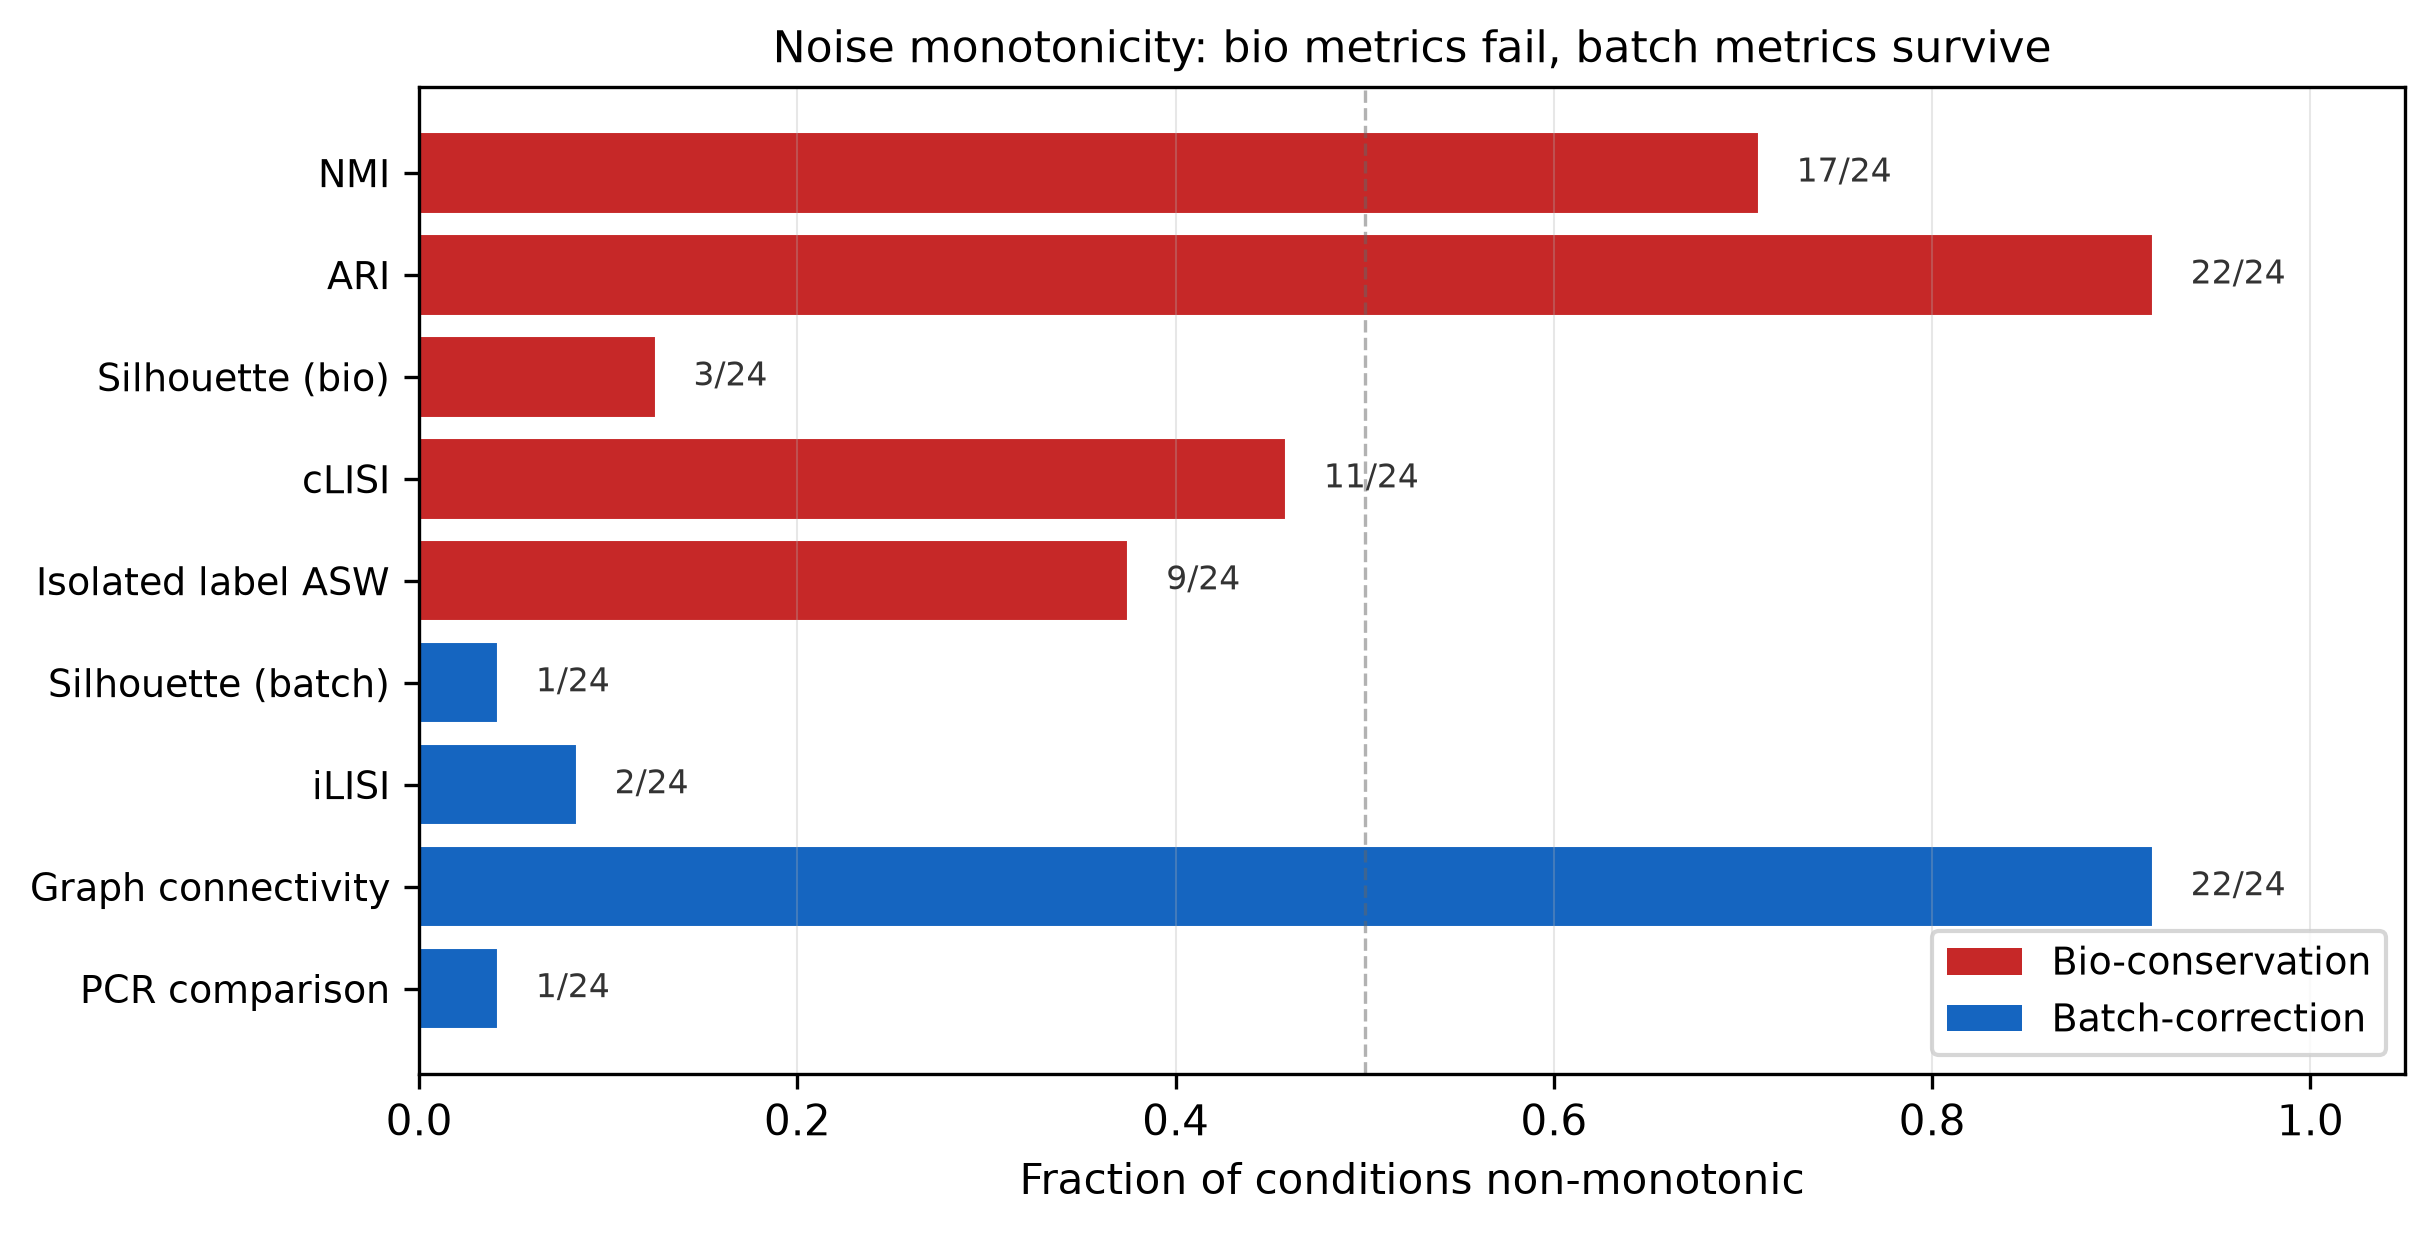
\includegraphics[width=0.75\textwidth]{figures/monotonicity_summary.pdf}
\caption{Non-monotonic fraction per metric (out of 24 conditions). Bio-conservation metrics (red): 3/24 to 22/24. Batch-correction metrics (blue): $\leq$2/24 except graph connectivity (22/24). kBET omitted (all null).}
\label{fig:monotonicity}
\end{figure}

\begin{figure}[htb]
\centering
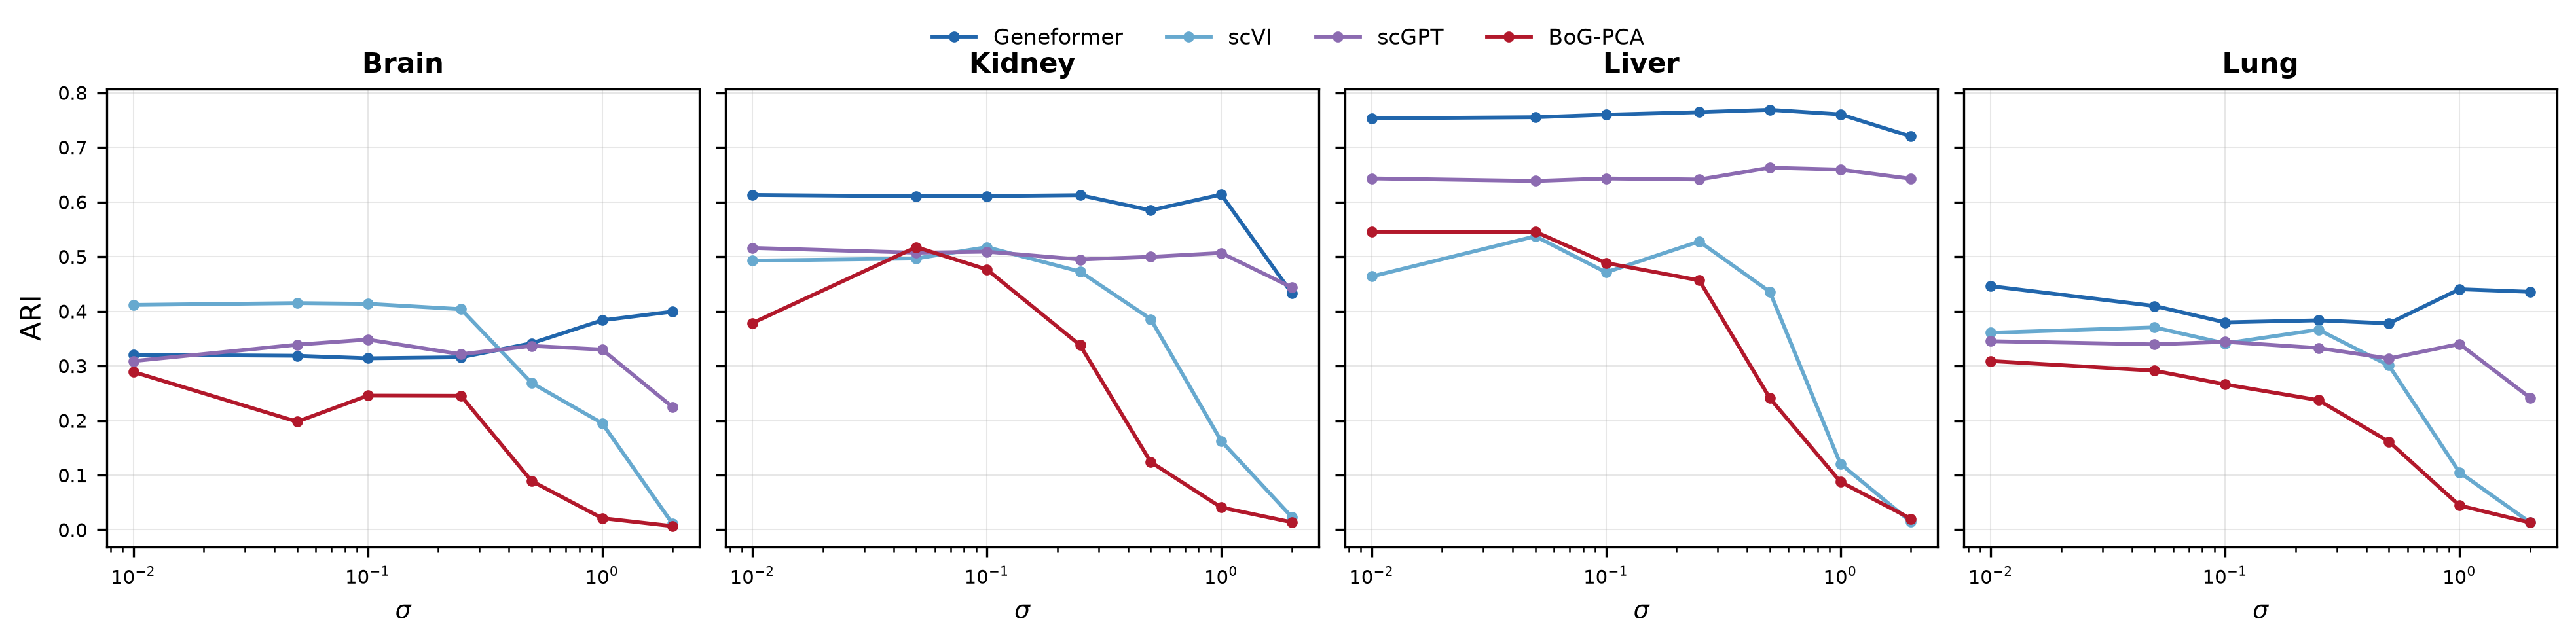
\includegraphics[width=\textwidth]{figures/noise_all_tissues.pdf}
\caption{ARI dose-response across all four tissues. Non-monotonicity is universal: every tissue shows at least one embedding with an initial plateau or increase before collapse. Geneformer is most robust; BoG-PCA collapses fastest.}
\label{fig:noise_tissues}
\end{figure}

\bibliographystyle{plainnat}
\bibliography{paper_d_v11}

\end{document}
